\PassOptionsToPackage{dvipsnames}{xcolor}
\documentclass[11pt]{article}
\usepackage[a4paper,margin=22mm]{geometry}
\usepackage[no-math]{fontspec}
\setmainfont{DejaVu Serif}
\usepackage{amsmath,amssymb,amsthm,mathtools,graphicx,xcolor,hyperref,xurl,xspace,ifthen,enumerate}
\setlength{\emergencystretch}{4em}
\AtBeginDocument{\special{pdf:mapline pzdr Dingbats <uzdr.pfb}}
\SetMathAlphabet{\mathbf}{normal}{OT1}{cmr}{bx}{n}
\SetMathAlphabet{\mathbf}{bold}{OT1}{cmr}{bx}{n}
\newtheorem{theo}{Theorem}[section]
\newtheorem{lemm}[theo]{Lemma}
\newtheorem{thm}[theo]{Theorem}
\newtheorem{proposition}[theo]{Proposition}
\newtheorem{corollary}[theo]{Corollary}
\newtheorem{definition}[theo]{Definition}
\newtheorem{theorem}[theo]{Theorem}
\newtheorem*{remas*}{Remarks}
\newtheorem{remas}[theo]{Remarks}
\newtheorem*{exam*}{Example}
\newtheorem{ques}[theo]{Question}
\providecommand{\og}{«\nobreakspace}
\providecommand{\fg}{\nobreakspace»}
\newtheorem{lem}[theo]{Lemma}
\newtheorem{lemma}[theo]{Lemma}
\newtheorem{prop}[theo]{Proposition}
\newtheorem{coro}[theo]{Corollary}
\newtheorem{corol}[theo]{Corollary}
\newtheorem*{conj*}{Conjecture}
\newtheorem{conj}[theo]{Conjecture}
\newtheorem{conjecture}[theo]{Conjecture}
\newtheorem{Proposition}[theo]{Proposition}
\newtheorem{theoreme}[theo]{Theorem}
\theoremstyle{definition}
\newtheorem{defi}[theo]{Definition}
\newtheorem{exam}[theo]{Example}
\newtheorem{exem}[theo]{Example}
\newtheorem{remark}[theo]{Remark}
\newtheorem{example}[theo]{Example}
\newtheorem{rema}[theo]{Remark}
\newtheorem{nota}[theo]{Notation}
\newtheorem{notation}[theo]{Notation}
\newtheorem{question}[theo]{Question}
\newtheorem*{rema*}{Remark}
\newtheorem*{defi*}{Definition}
\newtheorem*{theo*}{Theorem}
\newtheorem*{lemm*}{Lemma}
\newtheorem*{prop*}{Proposition}
\newcommand{\enoncename}{}
\newtheorem{corpusenonce}[theo]{\enoncename}
\newenvironment{enonce}[2][]{\renewcommand{\enoncename}{#2}\begin{corpusenonce}}{\end{corpusenonce}}
\newenvironment{enonce*}[2][]{\par\medskip\noindent\textbf{#2.}\itshape}{\par\medskip}
\newenvironment{proofc}[1][\proofname]{\begin{proof}[#1]}{\end{proof}}
\newcommand{\Mc}{\mathcal{M}}
\newcommand{\pointir}{.\ ---\ }
\newcommand{\equalenv}[2]{\expandafter\let\csname#1\expandafter\endcsname\csname#2\endcsname\expandafter\let\csname end#1\expandafter\endcsname\csname end#2\endcsname}
\providecommand{\diagbox}[3][]{\begin{tikzpicture}[x=1em,y=1em,baseline=(current bounding box.center)]\useasboundingbox(0,0) rectangle(3,1.4);\draw(0,1.4)--(3,0);\node at(.5,.3){#2};\node at(2.5,1.1){#3};\end{tikzpicture}}
\providecommand{\eg}{e.g.\ }
\providecommand{\ie}{i.e.\ }

\providecommand{\mathof}[1]{\mathrm{#1}}

\numberwithin{equation}{section}


\def\endappendix{}
\let\fg\undefined


% Unused stackengine import omitted; no stackengine macro occurs in retained Sections1--9.
\usepackage{tikz}
\usetikzlibrary{intersections,calc,arrows.meta}
% Unused youngtab import omitted; no youngtab macro occurs in retained Sections1--9.
% Unused ytableau import omitted; no tableau macro occurs in retained native body.
\usepackage[position=bottom]{subfig}
\allowdisplaybreaks
\usepackage[all]{xy}
\usepackage{amscd,epsfig}
\usepackage[nameinlink]{cleveref}

\equalenv{defin}{defi}
\equalenv{corol}{coro}


\Crefname{lemm}{Lemma}{Lemmata}
\Crefname{theo}{Theorem}{Theorems}
\Crefname{defi}{Definition}{Definitions}
\Crefname{exam}{Example}{Examples}
\Crefname{rema}{Remark}{Remarks}
\Crefname{coro}{Corollary}{Corollaries}
\Crefname{prop}{Proposition}{Propositions}


\newcommand{\nc}{\newcommand}
\nc{\rnc}{\renewcommand}

\nc{\bb}[1]{{\mathbb #1}}
\nc{\bbA}{\bb{A}}\nc{\bbB}{\bb{B}}\nc{\bbC}{\bb{C}}\nc{\bbD}{\bb{D}}
\nc{\bbE}{\bb{E}}\nc{\bbF}{\bb{F}}\nc{\bbG}{\bb{G}}\nc{\bbH}{\bb{H}}
\nc{\bbI}{\bb{I}}\nc{\bbJ}{\bb{J}}\nc{\bbK}{\bb{K}}\nc{\bbL}{\bb{L}}
\nc{\bbM}{\bb{M}}\nc{\bbN}{\bb{N}}\nc{\bbO}{\bb{O}}\nc{\bbP}{\bb{P}}
\nc{\bbQ}{\bb{Q}}\nc{\bbR}{\bb{R}}\nc{\bbS}{\bb{S}}\nc{\bbT}{\bb{T}}
\nc{\bbU}{\bb{U}}\nc{\bbV}{\bb{V}}\nc{\bbW}{\bb{W}}\nc{\bbX}{\bb{X}}
\nc{\bbY}{\bb{Y}}\nc{\bbZ}{\bb{Z}}

\nc{\mbf}[1]{{\mathbf #1}}
\nc{\bfA}{\mbf{A}}\nc{\bfB}{\mbf{B}}\nc{\bfC}{\mbf{C}}\nc{\bfD}{\mbf{D}}
\nc{\bfE}{\mbf{E}}\nc{\bfF}{\mbf{F}}\nc{\bfG}{\mbf{G}}\nc{\bfH}{\mbf{H}}
\nc{\bfI}{\mbf{I}}\nc{\bfJ}{\mbf{J}}\nc{\bfK}{\mbf{K}}\nc{\bfL}{\mbf{L}}
\nc{\bfM}{\mbf{M}}\nc{\bfN}{\mbf{N}}\nc{\bfO}{\mbf{O}}\nc{\bfP}{\mbf{P}}
\nc{\bfQ}{\mbf{Q}}\nc{\bfR}{\mbf{R}}\nc{\bfS}{\mbf{S}}\nc{\bfT}{\mbf{T}}
\nc{\bfU}{\mbf{U}}\nc{\bfV}{\mbf{V}}\nc{\bfW}{\mbf{W}}\nc{\bfX}{\mbf{X}}
\nc{\bfY}{\mbf{Y}}\nc{\bfZ}{\mbf{Z}}

\nc{\bfa}{\mbf{a}}\nc{\bfb}{\mbf{b}}\nc{\bfc}{\mbf{c}}\nc{\bfd}{\mbf{d}}
\nc{\bfe}{\mbf{e}}\nc{\bff}{\mbf{f}}\nc{\bfg}{\mbf{g}}\nc{\bfh}{\mbf{h}}
\nc{\bfi}{\mbf{i}}\nc{\bfj}{\mbf{j}}\nc{\bfk}{\mbf{k}}\nc{\bfl}{\mbf{l}}
\nc{\bfm}{\mbf{m}}\nc{\bfn}{\mbf{n}}\nc{\bfo}{\mbf{o}}\nc{\bfp}{\mbf{p}}
\nc{\bfq}{\mbf{q}}\nc{\bfr}{\mbf{r}}\nc{\bfs}{\mbf{s}}\nc{\bft}{\mbf{t}}
\nc{\bfu}{\mbf{u}}\nc{\bfv}{\mbf{v}}\nc{\bfw}{\mbf{w}}\nc{\bfx}{\mbf{x}}
\nc{\bfy}{\mbf{y}}\nc{\bfz}{\mbf{z}}


\nc{\mcal}[1]{{\mathcal #1}}
\nc{\calA}{\mcal{A}}\nc{\calB}{\mcal{B}}\nc{\calC}{\mcal{C}}\nc{\calD}{\mcal{D}}
\nc{\calE}{\mcal{E}} \nc{\calF}{\mcal{F}}\nc{\calG}{\mcal{G}}\nc{\calH}{\mcal{H}}
\nc{\calI}{\mcal{I}}\nc{\calJ}{\mcal{J}}\nc{\calK}{\mcal{K}}\nc{\calL}{\mcal{L}}
\nc{\calM}{\mcal{M}}\nc{\calN}{\mcal{N}}\nc{\calO}{\mcal{O}}\nc{\calP}{\mcal{P}}
\nc{\calQ}{\mcal{Q}}\nc{\calR}{\mcal{R}}\nc{\calS}{\mcal{S}}\nc{\calT}{\mcal{T}}
\nc{\calU}{\mcal{U}}\nc{\calV}{\mcal{V}}\nc{\calW}{\mcal{W}}\nc{\calX}{\mcal{X}}
\nc{\calY}{\mcal{Y}}\nc{\calZ}{\mcal{Z}}

\nc{\fA}{\mathfrak{A}}\nc{\fB}{\mathfrak{B}}\nc{\fC}{\mathfrak{C}} \nc{\fD}{\mathfrak{D}}
\nc{\fE}{\mathfrak{E}}\nc{\fF}{\mathfrak{F}}\nc{\fG}{\mathfrak{G}}\nc{\fH}{\mathfrak{H}}
\nc{\fI}{\mathfrak{I}}\nc{\fJ}{\mathfrak{J}}\nc{\fK}{\mathfrak{K}}\nc{\fL}{\mathfrak{L}}
\nc{\fM}{\mathfrak{M}}\nc{\fN}{\mathfrak{N}}\nc{\fO}{\mathfrak{O}}\nc{\fP}{\mathfrak{P}}
\nc{\fQ}{\mathfrak{Q}}\nc{\fR}{\mathfrak{R}}\nc{\fS}{\mathfrak{S}}\nc{\fT}{\mathfrak{T}}
\nc{\fU}{\mathfrak{U}}\nc{\fV}{\mathfrak{V}}\nc{\fW}{\mathfrak{W}}\nc{\fX}{\mathfrak{X}}
\nc{\fY}{\mathfrak{Y}}\nc{\fZ}{\mathfrak{Z}}

\nc{\fa}{\mathfrak{a}}\nc{\fb}{\mathfrak{b}}\nc{\fc}{\mathfrak{c}} \nc{\fd}{\mathfrak{d}}
\nc{\fe}{\mathfrak{e}}\nc{\fFf}{\mathfrak{f}}\nc{\fg}{\mathfrak{g}}\nc{\fh}{\mathfrak{h}}
\nc{\fri}{\mathfrak{i}}\nc{\fj}{\mathfrak{j}}\nc{\fk}{\mathfrak{k}}\nc{\fl}{\mathfrak{l}}
\nc{\fm}{\mathfrak{m}}\nc{\fn}{\mathfrak{n}}\nc{\fo}{\mathfrak{o}}\nc{\fp}{\mathfrak{p}}
\nc{\fq}{\mathfrak{q}}\nc{\fr}{\mathfrak{r}}\nc{\fs}{\mathfrak{s}}\nc{\ft}{\mathfrak{t}}
\nc{\fu}{\mathfrak{u}}\nc{\fv}{\mathfrak{v}}\nc{\fw}{\mathfrak{w}}\nc{\fx}{\mathfrak{x}}
\nc{\fy}{\mathfrak{y}}\nc{\fz}{\mathfrak{z}}

\newcommand{\Abb}{{\mathbb A}}
\newcommand{\C}{{\mathbb C}}
\newcommand{\bN}{{\mathbb{N}}}
\newcommand{\bQ}{{\mathbb{Q}}}
\newcommand{\bP}{{\mathbb{P}}}
\newcommand{\bR}{{\mathbb R}}
\newcommand{\T}{{\mathbb T}}
\newcommand{\bZ}{{\mathbb Z}}
\newcommand{\caD}{{\mathcal D}}
\newcommand{\cF}{{\mathcal F}}
\newcommand{\caH}{{\mathcal H}}
\newcommand{\caL}{{\mathcal L}}
\newcommand{\caF}{{\mathcal F}}
\newcommand{\cM}{{\mathcal M}}
\newcommand{\cO}{{\mathcal O}}
\newcommand{\cT}{{\mathcal T}}
\newcommand{\g}{\mathfrak{g}}
\newcommand{\Fl}{\mathrm{Fl}}
\newcommand{\Gr}{\mathrm{Gr}}

\newcommand{\aP}{\alpha}
\newcommand{\aX}{{\underline\alpha}}
\newcommand{\aPp}{{C(\alpha)}}
\newcommand{\csm}{c_{\mathrm{SM}}}
\newcommand{\ssm}{s_{\mathrm{M}}}
\newcommand{\csmv}{{c_{\text{SM},k}^\vee}}
\newcommand{\csmve}{{c_{\text{SM}}^\vee}}
\newcommand{\csmk}{{c_{\text{SM},k}}}
\newcommand{\csmh}{{c^\hbar_{\text{SM}}}}
\newcommand{\csT}{c^T_*}
\newcommand{\chcT}{\chc_*^T}
\newcommand{\csmhv}{{c^{\hbar,\vee}_{\text{SM}}}}
\newcommand{\csmT}{{c^T_{\text{SM}}}}
\newcommand{\csmTv}{{c^{T,\vee}_{\text{SM}}}}
\newcommand{\csmTk}{{c^T_{\text{SM},k}}}
\newcommand{\csmTh}{{c^{T,\hbar}_{\text{SM}}}}
\newcommand{\csmThv}{{c^{T,\hbar,\vee}_{\text{SM}}}}
\newcommand{\csmTvk}{{c^{T,\vee}_{\text{SM},k}}}
\newcommand{\cE}{\mathcal{E}}
\newcommand{\cQ}{\mathcal{Q}}
\newcommand{\cMa}{{c_{\text{Ma}}}}
\newcommand{\cMaTh}{{c_{\text{Ma}}^{T,\hbar}}}
\newcommand{\cMaT}{{c_{\text{Ma}}^{T}}}
\newcommand{\cMaTv}{{c^{T,\vee}_{\text{Ma}}}}
\newcommand{\chcMa}{\chc_{\text{Ma}}}
\newcommand{\chcMaT}{{\chc_{\text{Ma}}^T}}

\newcommand{\one}{1\hskip-3.5pt1}
\newcommand{\chc}{\check{c}}
\newcommand{\qede}{\hfill$\lrcorner$}
\newcommand{\Til}{\widetilde}
\newcommand{\cc}{\bold{c}}
\newcommand{\uX}{\underline X}
\newcommand{\h}{\mathrm{ht}}


\DeclareMathOperator{\id}{id}
\DeclareMathOperator{\rk}{rk}
\DeclareMathOperator{\CC}{CC}
\DeclareMathOperator{\DR}{DR}
\DeclareMathOperator{\Char}{Char}
\DeclareMathOperator{\Eu}{Eu}
\DeclareMathOperator{\cEu}{\check{E}u}
\DeclareMathOperator{\Shadow}{Shadow}
\DeclareMathOperator{\cn}{cn}
\DeclareMathOperator{\stab}{stab}
\DeclareMathOperator{\Lie}{Lie}
\DeclareMathOperator{\codim}{codim}
\DeclareMathOperator{\Pic}{Pic}
\DeclareMathOperator{\Frac}{Frac}
\DeclareMathOperator{\Ind}{Ind}
\DeclareMathOperator{\End}{End}
\DeclareMathOperator{\Hom}{Hom}
\DeclareMathOperator{\ch}{ch}
\DeclareMathOperator{\Attr}{Attr}
\DeclareMathOperator{\Slope}{Slope}
\DeclareMathOperator{\Deg}{Deg}
\DeclareMathOperator{\Supp}{Supp}
\DeclareMathOperator{\rank}{rank}
\DeclareMathOperator{\aff}{aff}
\DeclareMathOperator{\SL}{SL}
\DeclareMathOperator{\Red}{Red}
\DeclareMathOperator{\STab}{STab}
\DeclareMathOperator{\Stab}{Stab}
\DeclareMathOperator{\loc}{loc}
\DeclareMathOperator{\MPath}{MPath}
\DeclareMathOperator{\mult}{mult}
\DeclareMathOperator{\wt}{wt}
\DeclareMathOperator{\Sing}{Sing}


\begin{document}
\section*{\raggedright 626: Weighted Bruhat paths characterize Schubert smoothness}
\noindent\textbf{Author:} Mihalcea, Leonardo C.; Naruse, Hiroshi; Su, Changjian\par\noindent\textbf{Source:} Hook formulae from  Segre–MacPherson classes. Algebraic Combinatorics 8 (2025), publisher version, DOI 10.5802/alco.428. \url{https://alco.centre-mersenne.org/articles/10.5802/alco.428/}
\par\noindent\textbf{License:} CC BY 4.0, \url{https://creativecommons.org/licenses/by/4.0/}. The original publisher PDF cover has the explicit license notice. See the saved source/license records.
\par\noindent\textbf{Editorial material note (not author text):} The selected problem is Theorem9.1 for the exact parabolic quotient, interval and admissible Lambda weight: the weighted directed Bruhat path sum characterizes smoothness at the indicated Schubert point. The complete author Sections1--9 retain all local Segre-MacPherson localization/path recursion, equivariant Richardson CSM multiplicity and smoothness statements/proofs, and the Lambda-Bruhat graph/weight setup. Section10 illustrative Grassmannian/tableau examples are unselected and omitted; no tableau is altered or substituted. All retained diagrams are native editable TikZ/TeX. Named equivariant-geometric prerequisites remain explicit references. All proof text and formulas below are editable author TeX. Mathematical wording, language and proof order are retained. Only the article class, title matter and bibliography presentation are adapted for independent compilation; no proof has been generated or repaired.
\par\noindent\textbf{Editorial difficulty:} H2: The author argument constructs weighted Bruhat-path expressions for Segre–MacPherson localization and relates them to the smoothness criterion through equivariant multiplicities. Sections 5–8, particularly Theorem 7.5 and Proposition 8.12, retain the structural geometric and recursive coefficient arguments instead of assuming the desired path criterion.
\medskip\hrule\medskip
\noindent\textbf{Author statement, complete proof and local supporting text follow in source order.}
\section{Introduction} The goal of this paper is to reprove and generalize a version of 
Nakada's colored hook formula, using localization properties of the Segre--MacPherson 
classes of Schubert varieties. We recall first the version of Nakada's formula we generalize in this paper.

Let $G$ be a complex semisimple Lie group and fix opposite Borel groups $B,B^-$, giving  
$B \cap B^- = T$, a maximal torus in $G$. Let $R^+$ be the set of positive roots in~$B$, and let $W\coloneqq N_G(T)/T$ be
the Weyl group, endowed with the Bruhat order~$<$, and its length function $\ell: W \to \mathbb{N}$. For a Weyl 
group element $w \in W$, define the set~$S(w) = \{ \beta \in R^+: s_\beta w < w \}$. 

Let $w\in W$ be a $\pi$-minuscule Weyl group element for an integral dominant weight~$\pi$, in the sense of Peterson;
see~\cite{proctor:bruhat,carrell:vector,proctor:minuscule,stembridge:fullycomm,stembridge2001minuscule,graham.kreiman:cominuscule_pt} 
and \S\ref{sec:minuscule} below. Nakada's colored hook formula~\cite{nakada:colored} is the identity:
\begin{equation}\label{E:Nakada-intro}
	\sum \frac{1}{\beta_1}\cdot \frac{1}{\beta_1+\beta_2}\cdot \ldots \cdot\frac{1}{\beta_1+\beta_2+\cdots +\beta_r}
	=\prod_{\beta\in S(w)}\left(1+\frac{1}{\beta}\right) \/.
\end{equation}
Here the sum is over $r \ge 0$ and
oriented paths $x_r\overset{\beta_r}{\to} x_{r-1}\to \ldots \to x_1\overset{\beta_1}{\to} x_0=w$
in the Bruhat graph of the flag manifold $G/P$, where $P$ is the parabolic group with Weyl group $W_P = \Stab_W(\pi)$,
and the notation $x \overset{\beta}{\to} y$ means that $x,y $ are minimal length representatives such that 
$y W_P= s_\beta x W_P >xW_P$. See \S\ref{sec:hook} below for details. 

Nakada's formula is a vast generalization of several remarkable combinatorial formulae. One is the classical 
Frame--Robinson--Thrall hook formula calculating the dimension of the 
irreducible representation of the symmetric group $S_n$ indexed by the partition $\lambda$, or, equivalently, 
the number of standard tableaux of shape $\lambda$:
\begin{equation*}\label{equ:hook}
	\chi_\lambda(1)=\#\STab(\lambda)= \frac{n!}{\prod_{\square\in \lambda}h_\square} \/.
\end{equation*}
Here $h_\square$ is the hook length of a cell $\square$ in the Young diagram of $\lambda$. 
Another special case is
the Peterson formula counting the number $\#\Red(w)$ of reduced decompositions of a 
$\pi$-minuscule Weyl group element $w$:
\begin{equation}\label{E:introredw} \#\Red(w)=\frac{\ell(w)!}{\prod_{\beta\in S(w)}\h(\beta)} \/. \end{equation}
Here $\h(\alpha)$ denotes the height of the (positive) root $\alpha$, i.e., the sum of the coefficients
	of $\alpha$ when expanded in simple roots; see \S\ref{sec:prelims}.
We refer to~\cite{nakada:colored} or to \S\ref{sec:col-and-conseq} below for more details about how to obtain these specializations from Nakada's formula. 

Let $W^P$ be the set of minimal representatives for the quotient $W/W_P$. 
For each $w \in W^P$, denote by 
$Y(w)\coloneqq \overline{B^-w P/P} \subset G/P$ the corresponding Schubert variety.  
Our main goal is to prove an identity generalizing \Cref{E:Nakada-intro} in three directions:
\begin{enumerate}
	\item We remove the hypothesis that $w \in W$ is (Peterson) $\pi$-minuscule.
	\item We consider a `skew-version', for paths $v \le x_r \to \ldots \to x_0 = w$ where $v$ and $w$ are fixed, and such that 
	the Schubert variety $Y(v)$ is smooth at $w$. Nakada's formula is obtained from specializing $v=id$, 
	since $Y(id) = G/P$ is smooth at each $w$.
	\item Instead of fixing a single integral weight $\pi$, we consider an {\bf admissible weight function}
	$\Lambda: [v,w]^P \to {X^*(T)_P}$ from the Bruhat interval $[v,w]^P$ to the set of integral weights which stabilize $P$.
\end{enumerate}
The admissible functions are required to satisfy certain hypotheses spelled out in \S\ref{sec:LambdaBruhat}. 
An admissible function $\Lambda$ leads to a 
decorated version of the usual Bruhat graph which we call the {\bf $\Lambda$-Bruhat graph} of $G/P$.
This graph was used in~\cite{mihalcea:eqqgr,mihalcea:eqqhom} as part of an algorithm calculating the Schubert structure constants of the equivariant quantum cohomology ring of $G/P$.

A key observation going back to~\cite{mihalcea:eqqhom,naruse2014schubert,naruse2019skew} 
	is that the terms in special cases of Nakada's formula have geometric meaning, via
	localization properties of Schubert classes in equivariant cohomology
	and equivariant K-theory rings of flag manifolds. However, in order to obtain
	Nakada's formula \eqref{E:Nakada-intro}, a deformation of Schubert classes is needed.

Let $\csm(Y(v)) \in H^*_T(G/P)$ be the equivariant
Chern--Schwartz--MacPherson (CSM) class of the Schubert variety $Y(v)$. This class is defined using MacPherson's 
construction of characteristic classes of singular varieties~\cite{macpherson:chern}, generalized to the equivariant case by 
Ohmoto~\cite{ohmoto:eqcsm}; see \S\ref{sec:eqCSM}. Denote by 
\[ \ssm(Y(v)) = \frac{\csm(Y(v))}{c^T(T(G/P))} \in \widehat{H}^*_T(G/P) \]
the (equivariant) Segre--MacPherson (SM) class, which is an element in an 
appropriate completion of the equivariant cohomology ring. Let also 
$\ssm(Y(v))|_w \in H^*_T(pt)_{\loc}$ denote the localization of the SM class at the torus fixed point
$w \in G/P$. {(Here~$H^*_T(pt)_{\loc}$ is the fraction field of $H^*_T(pt)$.)}~Our 
most general result is the following; see \Cref{thm:smoothP} and \Cref{thm:LocCSM2}: 
	\begin{theorem}\label{thm:intro-main-rev}
		Let $v\leq  w\in W^P$, and fix an admissible 
		function $\Lambda:[v,w]^P\to X^{*}(T)_P$ with the associated 
		$\Lambda$-Bruhat graph $\Gamma$. Then: 
		\begin{equation}\label{intro:SMfrac} \sum\frac{m_\Lambda(x_r,x_{r-1})}{\mathcal{W}_\Lambda(x_r)}\cdot \frac{m_\Lambda(x_{r-1},x_{r-2})}{\mathcal{W}_\Lambda(x_{r-1})}\cdot \ldots \cdot \frac{m_\Lambda(x_{1},x_{0})}{\mathcal{W}_\Lambda(x_{1})}
			= 
			\frac{\ssm(Y(v))|_w}{\ssm(Y(w))|_w}\/. \end{equation}
		The sum is over integers $r \ge 0$, and over all directed paths 
		$v\leq x_r \overset{}{\to} x_{r-1} \overset{}{\to} \ldots \overset{}{\to} x_0 = w$ in $\Gamma$;
		$m_\Lambda(x,y) \in \bZ$ denotes the multiplicity of the edge $x \to y$; and $\mathcal{W}_\Lambda(x)
		\in X^{*}(T)_P$
		denotes the $\Lambda$-weight of $x$; see \Cref{def:ref_di} below. 
		
		Furthermore, set $S(w/v)\coloneqq \{\beta\in R^+\mid v\le s_\beta w<w\}$. Then:
		\[ \textrm{$Y(v)\subset G/P$ is smooth at $w\in G/P$} \Longleftrightarrow \frac{\ssm(Y(v))|_w}{\ssm(Y(w))|_w} = \prod_{\beta \in S(w/v)} \left(1+\frac{1}{\beta}\right) \/.\]
	\end{theorem}
	As a corollary we obtain a generalized version of Nakada's formula; cf.~\Cref{thm:genNak}:
	\begin{corol}\label{thm:intro-main} With the notation and hypotheses from the above theorem, 
		\begin{center}
			$Y(v)\subset G/P$ is smooth at $w\in G/P$  if and only if
			\begin{equation}\label{E:intro-main}
				\sum\frac{m_\Lambda(x_r,x_{r-1})}{\mathcal{W}_\Lambda(x_r)}\cdot \frac{m_\Lambda(x_{r-1},x_{r-2})}{\mathcal{W}_\Lambda(x_{r-1})}\cdot \ldots \cdot \frac{m_\Lambda(x_{1},x_{0})}{\mathcal{W}_\Lambda(x_{1})}
				\;=\;
				\prod_{\beta \in S(w/v)} \left(1+\frac{1}{\beta}\right) \/.\end{equation}
		\end{center}
\end{corol}
If $w$ is $\pi$-minuscule for a dominant integral weight $\pi$, and if the admissible function
is constant $\Lambda \equiv \pi$ on the interval $[v,w]^P$,
then each multiplicity $m_\Lambda(x_{i},x_{i-1})=1$, and one obtains 
a skew generalization of Nakada's identity \eqref{E:Nakada-intro}; see \Cref{col:Nak} below. 
The proof of this ultimately requires a 
good understanding of the (paths in the) interval $[v,w]^P$ for $\pi$-minuscule elements $v,w$, in analogy to 
the intervals in the Young lattice; for instance, the intervals in the weak and strong Bruhat order
coincide. We refer to \S\ref{sec:minuscule-intervals} and \S\ref{sec:genhook} 
for more details. We encourage the reader to jump to \S10, where we give some 
	examples illustrating this theorem.

Equation \eqref{intro:SMfrac} is proved by utilizing a Molev--Sagan type recursion~\cite{molev.sagan:Littlewood-Richardson}, based on a Chevalley formula to multiply SM classes; 
cf.~\Cref{lem:recLR} and see also~\cite{su:quantum,AMSS:shadows}. Variants of this recursion have been successfully used in~\cite{knutson.tao:puzzles,
	mihalcea:eqqgr,mihalcea:eqqhom,naruse2014schubert,BCMP:QKChev,naruse2019skew}
to study properties of the {\em equivariant} (quantum) cohomology or K-theory of flag manifolds. As a by-product of this study, and in the same spirit as the references
above, we obtain an algorithm for the structure constants of the multiplication of SM classes; see \Cref{cor:SMLR} below. Different algorithms were also obtained in~\cite{su:structure}.

Once equation \eqref{intro:SMfrac} is proved, the second part of \Cref{thm:intro-main-rev} follows from a smoothness criterion of Schubert varieties 
in terms of localization of SM classes. {More precisely, if $R_w^v$ denotes the 
	Richardson variety, the fraction 
	\begin{equation*}\label{E:intro-eqmult} \frac{\ssm(Y(v))|_w}{\ssm(Y(w))|_w} = 
		e_{w,G/P} (\csm(R_w^{v})) \end{equation*}
	is equal to Brion's equivariant multiplicity~\cite{brion:eq-chow}
	of the CSM class of $R_w^v$;~cf.~\Cref{prop:eqmult}. 
	{From this perspective, the (generalized) Nakada's formula calculates the equivariant multiplicity of a Richardson variety.}    
	The smoothness of $Y(v)$ at $w$ ensures that the equivariant multiplicity is a product of factors corresponding to weights of the normal space of $Y(v)$ at $w$, and it leads to the right hand side of
	\eqref{E:intro-main}. Our smoothness criterion for $Y(v)$ at $w$ in \Cref{thm:smoothP} generalizes similar results about smoothness of Schubert varieties by Kumar~\cite{kumar1996nil} and Brion~\cite{brion:eq-chow}, the latter in terms of equivariant multiplicities. Our criterion is also related to the one from~\cite{AMSS:motivic} for motivic Chern classes of Schubert varieties, which has consequences in $p$-adic representation theory.} 

Among the consequences of \Cref{thm:intro-main} proved in section \S\ref{sec:col-and-conseq} 
we mention a skew version of the Peterson formula \eqref{E:introredw}; cf.~\Cref{cor:skewPP}.
\begin{corol} Take $v <w\in W$ be $\pi$-minuscule elements 
	such that $Y(v)$ is smooth at $w$. Recall that 
	$S(w/v)\coloneqq \{\beta\in R^+\mid v\le s_\beta w<w\}$.~Then:
	\begin{equation}\label{equ:petersonproctor-intro}
		\#\Red(wv^{-1})=\frac{(\ell(w)-\ell(v))!}{\prod_{\beta\in S(w/v)}\h(\beta)} ~\/.
	\end{equation}
\end{corol}
When considered in this generality, this corollary seems to be new. In type A, this formula has an interpretation as counting standard Young tableaux on the skew shape $w/v$, see~\cite{naruse2014schubert,morales.pak.panovaLhook,panova.petrov:hook}.
We will prove in a continuation of this work that this interpretation holds in other Lie types, and, furthermore, if $W$ is simply laced, the `skew' formula
	for $v<w$ is equal to the `straight' formula from \eqref{E:introredw}, applied to $id < wv^{-1}$.
	We also note that our general formula from \Cref{thm:intro-main-rev} implies a variant of the Corollary above
	which does not require smoothness; see \Cref{rem:general_miuscule} below.

\Cref{thm:intro-main-rev} is the prototype of more general results. For instance,
a similar theorem - with essentially the same proof - may be obtained if one replaces the (cohomological) SM classes
with their K-theoretic versions, the {\em motivic Segre classes} of Schubert varieties~\cite{AMSS:motivic,mihalcea2020left}.
Because of the
technical challenges (in geometry and combinatorics) when working in K-theory, this will be studied
in separate work. Furthermore, there are versions of
Nakada's colored hook formula~\cite{nakada:colored} which hold in the Kac--Moody setting, 
suggesting that analogues of  
\Cref{thm:intro-main-rev} might exist in that generality as well.\begin{footnote} 
{After this paper was written, a generalization to arbitrary Coxeter groups Nakada's formula from \Cref{thm:anotherform} was proved in
\cite{MNS24Coxeterhook}.}\end{footnote}


\section{Preliminaries}\label{sec:prelims}
We start by fixing the notation used throughout the paper. Let $G$ be a simply connected complex 
Lie group with Borel subgroup $B$ and maximal torus $T\subset B$. Denote by 
$\mathrm{Lie}(G)$ and by 
$\mathrm{Lie}(T)$ 
be corresponding Lie algebras. Let 
$R^+\subset \mathrm{Lie}(T)^*\coloneqq \mathrm{Lie}(T)^*_\bbQ$
denote the positive roots, 
i.e those roots in $B$, and by $\Sigma =\{ \alpha_i: i \in I \}$ the set of simple roots. Let 
$\h: R^+ \to \mathbb{Z}$ 
denote the height function, defined by $\h(\sum a_i \alpha_i) = \sum a_i$. Let $R\coloneqq R^+\sqcup -R^+$. 
We use $\alpha>0$ (resp.~$\alpha<0$) to denote $\alpha\in R^+$ (resp. $\alpha\in -R^+$). For any 
root $\alpha\in R$, let 
$\alpha^\vee \subset \mathrm{Lie}(T)$
denote the corresponding coroot. Let~$\langle \cdot,\cdot \rangle: \mathrm{Lie}(T)^{*}\times \mathrm{Lie}(T)\to \bbQ$
denote the usual pairing, and let 
$X^*(T)\subset \mathrm{Lie}(T)^*$ 
be the (integral) weight lattice. 
Let $\{\varpi_i\mid i\in I\}\subset X^*(T)$ be the fundamental weights; they satisfy $\langle \varpi_i, \alpha_j^\vee \rangle = \delta_{i,j}$.
The Weyl group $W = N_G(T)/T$ is generated by simple reflections $s_i= s_{\alpha_i}$ ($i \in I$), and it is equipped with 
the Bruhat order $\leq$; we denote by~$w_0$ the longest element. For any $w\in W$, let $\Red(w)$ 
denote the set of all the reduced expressions for $w$. For $v < w \in W$, define 
\begin{equation}\label{equ:wvinversion}
	S(w/v)\coloneqq \{\beta\in R^+\mid v\le s_\beta w<w\}.
\end{equation}
If $v=id$, we denote $S(w/id)$ by $S(w)$.

Let $P (\supseteq B)$ be a parabolic subgroup with simple roots $\Sigma_P\subset \Sigma$ in $P$. This determines
the set $R_P^+ \subset R^+$ of those positive roots spanned by $\Sigma_P$, and the subgroup $W_P \subset W$ generated 
by the simple reflections $s_i$ where $\alpha_i \in \Sigma_P$. Denote by $W^P$ the set of 
minimal length representatives in $W/W_P$. The elements $w\in W^P$ are characterized by the property that $w(R^+_P)\subset R^+$. 
The torus fixed points $(G/P)^T$ are $\{wP\mid w\in W^P\}$. For any $w\in W^P$, let 
$T_w(G/P)$ denote the tangent space at $wP$. For any $w\in W$, let $X(w)^\circ\coloneqq BwP/P\subset G/P$ (resp. 
$Y(w)^\circ\coloneqq B^-wP/P\subset G/P$) denote the Schubert cell with closure $X(w)$ (resp. $Y(w)$), where 
$B^-$ is the opposite Borel subgroup. In particular, $X(w)^\circ=X(u)^\circ$ when the two cosets $wW_P$ and 
$uW_P$ are equal to each other. The Bruhat order restricts to the (Bruhat) order
on the cosets 
$\{wW_P\mid w\in W^P\}$, and it characterized by $uW_P\leq wW_P$ if and only if 
$uP\in X(w)$. Let $X^{*}(T)_P\coloneqq \{\lambda\in X^{*}(T)\mid \langle\lambda, \gamma^\vee\rangle=0 \text{ for all }
\gamma\in R^+_P \}$ be the set of integral weights which vanish on $ (R^+_P)^\vee$. For any 
$\lambda\in X^*(T)_P$, let $\calL_\lambda$ denote the line bundle $G\times^P\bbC_\lambda\in\Pic(G/P)$, which has 
fibre over $1.P$ the $T$-module of weight $\lambda$.

Let $H_T^*(G/P)$ denote the equivariant cohomology of the partial flag variety $G/P$. It has a basis of the Schubert classes:
\[H_T^*(G/P)=\bigoplus_{w\in W^P} H_T^*(pt)[X(w)]=\bigoplus_{w\in W^P} H_T^*(pt)[Y(w)],\]
{where $[X(w)]$ and $[Y(w)]$ denote the Poincar{\'e} dual of the fundamental classes of the Schubert varieties.}
For any $\kappa \in H_T^*(G/P)$ and $w\in W^P$, let $\kappa|_w\in H_T^*(pt)$ denote the restriction of $\kappa$ to the fixed point $wP\in G/P$.
Let $H_T^*(G/P)_{\loc} \coloneqq H_T^*(G/P)\otimes_{H_T^*(pt)}\Frac H_T^*(pt)$ be the localized equivariant cohomology of $G/P$, where $\Frac H_T^*(pt)$ denotes the fraction field of $H_T^*(pt)$. 
By the localization theorem,  $H_T^*(G/P)_{\loc}$ has a basis formed by the classes of fixed points $\{[wP]\mid w\in W^P\}$; 
this is called the fixed point basis.  

The Weyl group $W$ acts on $G/P$ by left multiplication. It induces an action of $W$ on $H_T^*(G/P)$, 
which acts on the base ring 
$H_T^*(pt)=Sym_{\mathbb{Z}}(X^*(T))$
by the usual Weyl group action. Let $\varphi_{w_0}$ denote the action induced by 
the longest Weyl group element. Then $\varphi_{w_0}([X(w)])=[Y(w_0w)]$.

{This paper will focus on Peterson, or $\pi$-minuscule, elements, for some 
dominant integral weight $\pi$. Before giving the formal definition in 
\Cref{sec:minuscule}, we note that the Schubert varieties indexed by $\pi$-minuscule elements
share most geometric and combinatorial properties of the Schubert varieties in Grassmannians, or, 
more generally, in (co)minuscule Grassmannians.\begin{footnote}{Aside from the ordinary Grassmannians, 
the list of minuscule Grassmannians includes the maximal orthogonal 
Grassmannians in Lie type D, even quadrics, the Cayley plane in type $E_6$, 
and the Freudenthal variety in type $E_7$. If, as in this paper, one distinguishes the data of torus actions, 
then the projective spaces $\bP^{2n-1} \simeq \mathrm{IG}(1,2n)$ in types A and C, and the maximal orthogonal 
Grassmannians $\mathrm{OG}(n,2n+1)\simeq \mathrm{OG}(n+1,2n+2)$ in types B and D are listed as 
separate varieties.}\end{footnote} In fact, any Schubert variety in a cominuscule
Grassmannian $G/P$ is indexed by a $\pi$-minuscule element, for $\pi$ the fundamental weight 
associated to the parabolic subgroup $P$. As a first approximation, the reader may 
consider $\pi$-minuscule elements as generalizing the usual Young diagrams for Grassmannians,
or the more general Young diagrams defined by Proctor~\cite{proctor:bruhat,proctor:minuscule}, and Stembridge~\cite{stembridge:fullycomm,stembridge2001minuscule} (see also~\cite{graham.kreiman:cominuscule_pt}) in other Lie types.
}


\section{Nakada's colored hook formula}\label{sec:hook}
In this section, we review Nakada's colored hook formula from~\cite{nakada:colored,nakada:proc}. This formula generalizes results of Proctor 
\cite{proctor:minuscule,proctor:dynkin}
and D. Peterson (see e.g.~\cite{carrell:vector})
about the combinatorics of complete $d$-posets, and the number of reduced 
decompositions of certain minuscule Weyl group elements; see also~\cite{stanley:reduced}. 
In order to be able to use geometric arguments, in this paper we require that the Lie algebra of $G$
is of finite 
type, although Nakada's formula may be formulated for any Kac--Moody Lie algebra.


\subsection{Nakada's formula and pre-dominant weights}\label{sec:predominant} Recall that the integral weights
$\lambda \in \mathrm{Lie}(T)^*$
satisfy 
$\langle\lambda,\alpha_i^\vee\rangle\in \bZ$, for each $\alpha_i \in \Sigma$; a weight $\lambda$ is {\em dominant} if in addition $\langle\lambda,\alpha_i^\vee\rangle\geq 0$. Following 
\cite{nakada:colored}, we say that an integral weight $\lambda$ is {\em pre-dominant} if
$\langle \lambda, \beta^\vee\rangle \geq -1$ for all positive roots $\beta \in R^{+}$. For a pre-dominant integral weight $\lambda$, the {\em diagram} $D(\lambda)$ of $\lambda$ is defined by
\begin{equation}\label{diagram}
	D(\lambda)\coloneqq \{\beta\in R^{+} \mid \langle\lambda, \beta^\vee\rangle =-1\}.
\end{equation}
\noindent
If $\lambda$ is a dominant integral weight, it is pre-dominant, but $D(\lambda)=\emptyset$. 

We recall some elementary facts about pre-dominant integral weights from~\cite{nakada:colored}. 
\begin{lemma}[{\cite[Lemma 4.1]{nakada:colored}}]\label{lem:pre-dom}
	Let $\lambda$ be a pre-dominant integral weight. 
	
	
	(1) If $D(\lambda)\neq\emptyset$, then $D(\lambda) \cap \Sigma\neq \emptyset$.
	
	(2) For $\beta\in D(\lambda)$, $s_\beta(\lambda)$ is a pre-dominant integral weight.
	
	(3) In case (2), $D(s_\beta(\lambda))=s_\beta(D(\lambda)\setminus S(s_\beta))$.
\end{lemma}


For integral weights $\mu, \nu \in \fh^*$ and $\beta \in R^{+}$, define
\[\mu \overset{\beta}{\to} \nu \Longleftrightarrow \langle \mu, \beta^\vee\rangle=-1 \textit{ and } \nu=s_\beta(\mu) \/.\] In particular, if
$\mu \overset{\beta}{\to} \nu$ then $\nu = \mu + \beta$.

A $\lambda$-path of length $r$ is a sequence $(\beta_1,\beta_2,\ldots, \beta_r)$ where 
$$
\lambda=\lambda_0 \overset{\beta_1}{\to} \lambda_1 
\overset{\beta_2}{\to} \cdots
\overset{\beta_r}{\to} \lambda_r \/.
$$
We denote by ${\rm Path}(\lambda)$ the set of all $\lambda$-paths.
By \Cref{lem:pre-dom}(2), if $\lambda$ is pre-dominant, all the weights $\lambda_i$ in a $\lambda$-path are
pre-dominant. At each step in a $\lambda$-path, $|D(\lambda_i)|$ strictly decreases, therefore the 
length of a $\lambda$-path for a pre-dominant weight must be at most the size of $D(\lambda)$. 
Parts (1) and (3) of \Cref{lem:pre-dom} imply that a $\lambda$-path $(\beta_1, \ldots, \beta_d)$ of maximal length can only contain simple roots $\beta_i \in \Delta$, and that $d = |D(\lambda)|$. For a pre-dominant integral weight $\lambda$, 
we denote by ${\rm MPath}(\lambda)\subset {\rm Path}(\lambda)$ the subset of longest $\lambda$-paths.

Now we can state Nakada's colored hook formula.
\begin{theorem}[{Nakada's colored hook formula~\cite[Theorem 7.1]{nakada:colored}}]\label{thm:Nak}
	
	Let $\lambda$ be a pre-dominant integral weight. Then 
	$$
	\sum \frac{1}{\beta_1}\cdot \frac{1}{\beta_1+\beta_2}\cdot \ldots \cdot\frac{1}{\beta_1+\beta_2+\cdots +\beta_r}
	=\prod_{\beta\in D(\lambda)}\left(1+\frac{1}{\beta}\right) \/, 
	$$ where the sum is over all $r \ge 0$ and $\lambda$-paths $(\beta_1,\beta_2,\ldots,\beta_r)$.
\end{theorem}

Taking the lowest degree terms of the formula in \cref{thm:Nak},
we get the following corollary.
\begin{corol}[{\cite[Corollary 7.2]{nakada:colored}}]
	Let $\lambda$ be a pre-dominant integral weight and $d=|D(\lambda)|$.
	Then 
	$$
	\sum_{
		(\beta_{1},\beta_{2},\ldots,\beta_d)\in {\rm MPath}(\lambda)}
	\frac{1}{\beta_1}\cdot \frac{1}{\beta_1+\beta_2}\cdot \ldots \cdot\frac{1}{\beta_1+\beta_2+\cdots +\beta_d}
	=\prod_{\beta\in D(\lambda)}\frac{1}{\beta}.
	$$
\end{corol}
This formula generalizes the classical hook formula \eqref{equ:hook} and the Peterson--Proctor formula \eqref{equ:petersonproctor-intro}; see also \S\ref{sec:genhook} below. It is also related to an equality of rational functions involving root partitions for cluster variables cf.~\cite{Cas19,casbi2019newton}.

\subsection{Peterson minuscule elements}\label{sec:minuscule} 
For any integral weight $\pi$, D. Peterson defined the notion of a $\pi$-minuscule 
Weyl group element, see below and ~\cite{proctor:bruhat,carrell:vector,proctor:minuscule,stembridge:fullycomm,stembridge2001minuscule,graham.kreiman:cominuscule_pt}.
Examples of $\pi$-minuscule elements are the minimal length representatives in $W^P$, where
$P$ is the maximal parabolic associated to a minuscule fundamental weight.~{Minuscule elements are fully commutative
	\cite{stembridge:fullycomm}; in particular, in type A they are $321$-avoiding.}
We will use this notion to rewrite Nakada's formula and its generalizations considered in this paper in terms of Weyl group elements. 
\begin{defin}[$\pi$-minuscule elements]\label{def:minuscule}
	Let $\pi$ be an integral weight.
	An element \mbox{$w\in W$} is called {\bf $\pi$-minuscule} if
	there is a reduced expression $w=s_{i_1} s_{i_2}\cdots s_{i_\ell}$ such that
	\begin{equation}\label{minuscule:1}
		\langle s_{i_{k+1}} s_{i_{k+2}}\cdots s_{i_\ell}(\pi), \alpha_{i_k}^\vee \rangle=1\hspace{1cm} (1\leq k\leq \ell)
	\end{equation}
	Equivalently, 
	\begin{equation}\label{equ:actiononmin}
		s_{i_k} s_{i_{k+1}} s_{i_{k+2}}\cdots s_{i_\ell}(\pi) = \pi - \alpha_{i_\ell} - \ldots - \alpha_{i_k}.
	\end{equation}
\end{defin}
From the definition it follows that if $w$ is $\pi$-minuscule, then its length is $\ell(w) = \h(\pi- w(\pi))$.  
The next result follows immediately from analyzing the inversion set of~$w$. 
\begin{lemma}[{\cite[Proposition 5.1]{stembridge2001minuscule}}]\label{lem:gamma}
	If $w\in W$ then
	\begin{center}
		$w$ is $\pi$-minuscule $\iff$ $\langle\pi, \gamma^\vee\rangle=1$ for all $\gamma\in R^{+}$
		such that $w s_\gamma <w$.
	\end{center}
\end{lemma}
From now on we restrict to the case when $\pi$ is a a dominant integral weight. Let~$W_\pi=\Stab_W(\pi)$ denote the stabilizer subgroup of $\pi$ inside $W$. This determines the parabolic subgroup $P$ such that $W_P=W_\pi$, containing simple roots \mbox{$\Sigma_P\coloneqq \{\alpha_i\in \Sigma\mid \langle \pi,\alpha_i^\vee\rangle=0\}$}. Let $W^\pi$ denote the set of minimal length representatives for the cosets $W/W_\pi$.
\begin{remark}\label{rem:wminuscule}
	It follows from \Cref{lem:gamma} that if $w$ is $\pi$-minuscule, then $w\in W^\pi$,
	and
	the property \eqref{minuscule:1} holds for any reduced expression 
	of $w=s_{i_1} s_{i_2}\cdots s_{i_\ell}$.
\end{remark}
We also need the following definition.
\begin{defin}\label{defin:order}
	For $u,w\in W^\pi$ and $\beta\in R^{+}$, define 
	\begin{equation*}\label{equ:order}
		u \overset{\beta}{\to} w \textit{\quad if \quad}  s_\beta wW_\pi=uW_\pi, \textit{ and }u<w.
	\end{equation*}
\end{defin}
\begin{lemma}\label{lemma:ubetav} Let $\pi$ be dominant integral and $u,w \in W^\pi$ such that 
	$u \overset{\beta}{\to} w$.~Then the following hold:
	
	(a) The root $\beta$ is unique.
	
	(b) There exists a unique positive root $\gamma$ such that $s_\beta w W_P = w s_\gamma W_P$.
	Furthermore, 
	\[ \gamma= - w^{-1}(\beta) \quad \textrm{ and } \quad ws_\gamma < w \/. \]
		
	(c) If in addition $w$ is $\pi$-minuscule then $\langle w(\pi), \beta^\vee \rangle = -1$.
\end{lemma}
\begin{proof} The uniqueness of $\beta$ follows from~\cite[Lemma 4.1]{fulton.woodward}. Since 
	$s_\beta w <w$ it follows that $w^{-1}(\beta)<0$, thus $\gamma\coloneqq  - w^{-1}(\beta)$ is a positive root,
	and $s_\gamma W_P = w^{-1} s_\beta w W_P = w^{-1} u W_P$. Since $w^{-1}u \notin W_P$ by hypothesis, the uniqueness of $\gamma$ follows from~\cite[Lemma 2.2]{buch.m:nbhds}. 
	Finally, since $ws_\gamma W_P = u W_P$ and $u <w$, then necessarily
	$ws_\gamma < w$. This finishes the proof of (b). Part (c) follows from (b) and \Cref{lem:gamma}.
\end{proof}


The relation between pre-dominant integral weights and $\pi$-minuscule elements is given by the following proposition.
\begin{prop}[{\cite[Propositions 10.1 and 10.3]{nakada:colored}}]\label{prop:pre-dom}
	There is a bijection between the following two sets
	\begin{align*}
		\{\textit{pre-dominant integral weights } \lambda\}&\\
		\longleftrightarrow  \{(\pi, w)\mid & \pi \textit{ is dominant integral, and }w \textit{ is } \pi \textit{-minuscule}\}.
	\end{align*}
	Here, $\lambda$ is determined by $(\pi,w)$ by the formula $\lambda=w(\pi)$.
	Conversely, for any pre-dominant integral weight $\lambda$,
	take a maximal $\lambda$-path 
	$(\alpha_{i_1},\alpha_{i_2},\ldots,\alpha_{i_d})\in {\rm MPath}(\lambda)$ and
	set $w=s_{i_1} s_{i_2}\cdots s_{i_d}$, $\pi=w^{-1}(\lambda)$.
	Then $\pi$ is a dominant integral weight and $w$ is $\pi$-minuscule.
	Moreover $D(\lambda)= S(w)=\{\beta\in R^{+}\mid s_\beta w<w\}$, and the correspondence $(\alpha_{i_1},\alpha_{i_2},\ldots,\alpha_{i_d})\mapsto s_{i_1} s_{i_2}\cdots s_{i_d}$ from ${\rm MPath}(\lambda)$ to $\Red(w)$ is bijective.
\end{prop}

\begin{corol}\label{lem:wminuscule}
	Let $\pi$ be a dominant integral weight, $w$ be $\pi$-minuscule and \mbox{$\lambda=w(\pi)$}. For $\beta\in R^+$, let $u\in W^\pi$ denote the minimal length representative in $s_\beta wW_\pi$. Then: 
	
	(a) $\lambda\overset{\beta}{\to} s_\beta(\lambda)$ is equivalent to $u \overset{\beta}{\to} w$.
	
	(b) If $u \overset{\beta}{\to} w$, then $u$ is also $\pi$-minuscule.
\end{corol}
\begin{proof} Part (a) follows from:
	{\small \[\lambda\overset{\beta}{\to} s_\beta(\lambda)\Leftrightarrow \langle\lambda,\beta^\vee\rangle=-1\Leftrightarrow \langle\pi,w^{-1}(\beta^\vee)\rangle=-1 \Leftrightarrow w^{-1}\beta<0\Leftrightarrow  s_\beta w<w\Leftrightarrow u\overset{\beta}{\to} w.\]}Here in the third equivalence, the $\Rightarrow$ direction follows from the fact that $\pi$ is dominant, while the $\Leftarrow$ direction follows from \Cref{lemma:ubetav}. 
	
	To prove (b), observe that if $u\overset{\beta}{\to} w$, then $s_\beta\lambda$ is also a pre-dominant integral weight by \Cref{lem:pre-dom}(2). Because of \Cref{prop:pre-dom},
	\[s_\beta\lambda=w'(\pi')\]
	for some dominant integral weight $\pi'$, $w'\in W$ such that $w'$ is $\pi'$-minuscule. Therefore,
	\[s_\beta w(\pi)=w'(\pi') \/,\]
	and because the dominant 
	weights $\pi, \pi'$ are in the fundamental 
	domain for the $W$-action, it follows that $\pi=\pi'$, and that $s_\beta wW_\pi=w'W_\pi$. By \Cref{rem:wminuscule}, $w'\in W^\pi$. Thus, $w'=u$, and $u$ is $\pi$-minuscule.
\end{proof}

With \Cref{lem:wminuscule}, Nakada's formula (\Cref{thm:Nak}) can be reformulated as follows.
\begin{theorem}[Nakada]\label{thm:anotherform}
	Let $\pi$ be a dominant integral weight, and $w\in W$ be a $\pi$-minuscule element. Then: 
	\[ \sum \frac{1}{\beta_1}\cdot \frac{1}{\beta_1+\beta_2}\cdot \ldots \cdot\frac{1}{\beta_1+\beta_2+\cdots +\beta_r}
	=\prod_{\beta\in S(w)}\left(1+\frac{1}{\beta}\right) \/,
	\] where the summation is over $r \ge 0$ and paths $x_r\overset{\beta_r}{\to} x_{r-1}\to \ldots \to x_1\overset{\beta_1}{\to} x_0=w$.
	In particular, 
	$$
	{\sum_{x_d\overset{\beta_d}{\to} x_{d-1}\to \ldots \to x_1\overset{\beta_1}{\to} x_0=w\/}}
	\frac{1}{\beta_1}\cdot \frac{1}{\beta_1+\beta_2}\cdot \ldots \cdot \frac{1}{\beta_1+\beta_2+\cdots +\beta_d}
	=\prod_{\beta\in S(w)}\frac{1}{\beta},
	$$
	where $d=|S(w)|{= \ell(w)}$.
\end{theorem}
This statement will generalized in \Cref{col:Nak} below.

\subsection{Bruhat intervals of \texorpdfstring{$\pi$}{pi}-minuscule elements}\label{sec:minuscule-intervals}
The main goal of this section is to prove \Cref{prop:weakstrong}, stating that the intervals in the weak and ordinary (or strong) Bruhat
order determined by two $\pi$-minuscule elements coincide. Special cases appeared
in the works by Stembridge~\cite[Thm.~7.1]{stembridge:fullycomm} (for $\pi$ a minuscule weight) and Proctor~\cite[\S 10]{proctor:minuscule} (for $G$ simply laced),
but we have not seen \Cref{prop:weakstrong} in the generality we need.

For $u,w \in W$ the (left) weak Bruhat order is defined by $u<_L w$ iff 
$\ell(wu^{-1}) = \ell(w) - \ell(u)$. Equivalently, $w=vu$ and $\ell(vu) = \ell(v) + \ell(u)$. 
Observe that if $u<_L w$ then $u<w$ in the strong Bruhat order, but in general the 
two orders are different. 
	\begin{example}
		Consider the example of type $A_2$. The Weyl group has two generators $s_1$, $s_2$. Let $w=s_1s_2$ and $u=s_1$. Then $u<w$, but $u \nless_L w$ as $\ell(wu^{-1}) \neq \ell(w)-\ell(u)$.
\end{example}
For $v<w\in W^P$, set $[v, w]^P\coloneqq \{x\in W^P\mid v\leq x\leq w\}$. 
\begin{prop}\label{prop:weakstrong} Let $\pi$ is a dominant integral weight 
	with $\Stab_W(\pi)=W_P$
	and let $u<w$ be $\pi$-minuscule elements in $W^P$. Then the interval
	$[u,w]^P \subset W^P$ is the same in the weak and strong Bruhat orders, i.e.,
	\[ \{ v \in W^P: u \le v \le w \} = \{ v' \in W^P: u \le_L v' \le_L w \} \/. \] 
\end{prop}
\begin{proof} Let $v \in W^P$ such that $v < w$. Then it suffices to show that 
	$v \le_L w$ when $w$ covers $v$ in the strong Bruhat order in $W^P$, i.e., 
	$\ell(w) - \ell(v) =1$. Write
	$v W_P= s_\beta w W_P = w s_\gamma W_P$ for positive roots $\beta, \gamma$ as in 
	\Cref{lemma:ubetav}. Since $w$ is $\pi$-minuscule, $v$ is also $\pi$-minuscule 
	by \Cref{lem:wminuscule} (b).
	Using that $\ell(w)= \h(\pi - w(\pi))$ we obtain 
	\[ 1 = \ell(w) - \ell(v) = \mathrm{ht}(s_\beta w(\pi) - w(\pi)) = 
	\h(w(\pi) - \langle w(\pi), \beta^\vee\rangle \beta - w(\pi)) = \h(\beta) \/.\]
	The last equality follows because the multiplicity $\langle w(\pi), \beta^\vee\rangle =-1$ 
	by \Cref{lemma:ubetav}(c). Therefore $\beta$ must be a simple root, and, furthermore, $w=s_\beta v$,
	thus $v \le_L w$. 
\end{proof}
The special case $u=id$ of the following corollary has been proved by Nakada
\cite[Proposition 10.3]{nakada:colored}.
\begin{corol}\label{cor:skewred} Assume the hypotheses from \Cref{prop:weakstrong}. Let \mbox{$d\coloneqq  \ell(w)-\ell(u)$}.
	There is a bijection between the set of reduced words of $wu^{-1}$ and the set of maximal length
	paths from $u$ to $w$, {sending a reduced word $wu^{-1} = s_{\beta_1} \cdot \ldots \cdot s_{\beta_d}$ to} the path
	\[ u=x_d\overset{\beta_d}{\to} x_{d-1}\to \ldots \to x_1\overset{\beta_1}{\to} x_0=w \/. \]
\end{corol}
\begin{proof} Consider any path 
	$u=x_d\overset{\beta_d}{\to} x_{d-1}\to \ldots \to x_1\overset{\beta_1}{\to} x_0=w$
	in the (strong) Bruhat interval $[u,w]^P$. Then $\ell(x_{i-1}) - \ell(x_{i}) = 1$ for all $i$, and
	since $w$ is $\pi$-minuscule all $x_i$'s must be also. Because weak and strong 
	Bruhat orders coincide in $[u,w]^P$ by \Cref{prop:weakstrong},
	$x_{i} = s_{\beta_i} x_{i-1}$ and each of the roots $\beta_i$ must be simple. Then
	$s_{\beta_d}s_{\beta_{d-1}} \cdot \ldots \cdot s_{\beta_1}= uw^{-1}$ and this decomposition
	is reduced. This associates a reduced word of $wu^{-1}$ to the given path (by reading in reverse), 
	and it easily follows that this correspondence is a bijection.\end{proof}

\section{Chern--Schwartz--MacPherson classes of Schubert cells}\label{sec:eqCSM}
In this section, we recall the definition of the equivariant Chern--Schwartz--MacPherson (CSM) and Segre--MacPherson (SM) classes, 
then we recall the Chevalley formula for the CSM and SM classes of Schubert cells in partial flag manifolds~\cite{AMSS:shadows,su:quantum}.

\subsection{Definition}
Let $X$ be a complex algebraic variety. The group of constructible functions $\calF(X)$ consists of functions $\varphi = \sum_W c_W \one_W$, where the sum is over a finite set of constructible subsets $W \subset X$,
$c_W \in \bbZ$ are integers, and $\one_W$ is the characteristic function of $W$.
For a proper morphism $f:Y\rightarrow X$, there is a linear map \mbox{$f_*:\calF(Y)\rightarrow \calF(X)$}, such that for any constructible subset $W\subset Y$, we have $f_*(\one_W)(x)=\chi_{\textit{top}}(f^{-1}(x)\cap W)$, where $x\in X$ and $\chi_{\textit{top}}$ denotes the topological Euler characteristic.
Thus $\calF$ can be considered as a (covariant) functor from the category of complex algebraic varieties and 
proper morphisms to the category of abelian groups.

According to a conjecture attributed to Deligne and Grothendieck, there is a unique natural transformation $c_*: \calF \to H_*$ from the functor of constructible functions on a complex algebraic variety $X$ to the homology functor, where all morphisms are proper, such that if $X$ is smooth then $c_*(\one_X)=c(TX)\cap [X]$, {where $c(TX)$ denotes the total Chern class of the tangent bundle $TX$ and $[X]$ denotes the fundamental class}.  This conjecture was proved by MacPherson~\cite{macpherson:chern}; the class $c_*(\one_X)$ for possibly singular $X$ was shown to coincide with a class defined earlier by M.-H.~Schwartz~\cite{schwartz:1, schwartz:2, BS81}. 

The theory of CSM classes was later extended to the equivariant setting by Ohmoto~\cite{ohmoto:eqcsm}. If $X$ has an 
action of a torus $T$, Ohmoto defined the group $\calF^T(X)$ of {\em equivariant\/} constructible functions. 
We will need the following properties of this group: 
\begin{enumerate} 
	\item If $W \subseteq X$ is a constructible set which is invariant under the $T$-action, its characteristic function $\one_W$ is an element of $\calF^T(X)$. We will denote by $\calF_{inv}^{T}(X)$ the subgroup of $\calF^{T}(X)$ consisting of $T$-invariant constructible functions on $X$. (The group $\cF^T(X)$ also contains other elements, but this will be immaterial for us.)
	\item Every proper $T$-equivariant morphism $f: Y \to X$ of algebraic varieties induces a homomorphism $f_*^T: \calF^T(X) \to \calF^T(Y)$. The restriction of $f_*^T$ to $\calF_{inv}^{T}(X)$ coincides with the ordinary push-forward $f_*$ of constructible functions. See~\cite[\S 2.6]{ohmoto:eqcsm}.
\end{enumerate}

Ohmoto proves~\cite[Theorem 1.1]{ohmoto:eqcsm} that there is an equivariant version of MacPherson transformation $c_*^T: \calF^T(X) \to H_*^T(X)$ that satisfies $c_*^T(\one_X) = c^T(TX) \cap [X]_T$ if~$X$ is a smooth variety, and that is functorial with respect to proper push-forwards. The last statement means that for all proper $T$-equivariant morphisms $Y\to X$ the following diagram
commutes:
$$\xymatrix{ 
	\calF^T(Y) \ar[r]^{c_*^T} \ar[d]_{f_*^T} & H_*^T(Y) \ar[d]^{f_*^T} \\ 
	\calF^T(X) \ar[r]^{c_*^T} & H_*^T(X).}$$ 
If $X$ is smooth, we will identify the (equivariant) homology and cohomology groups, 
by Poincar{\'e} duality: $H_*^T(X)\simeq H^*_T(X)$.


\begin{defin}
	Let $Z$ be a $T$-invariant constructible subvariety of $X$. 
	\begin{enumerate}
		\item
		We denote by $\csm(Z)\coloneqq c_*^T(\one_{Z}) {~\in H_*^T(X)}$ the {\em equivariant Chern--Schwartz--MacPherson (CSM) class\/} of $Z$. 
		\item 
		If $X$ is smooth, we denote by $\ssm(Z)\coloneqq \frac{c_*^T(\one_{Z})}{c^T(T X)} ~\in \widehat{H}^*_T(X)$ 
		the {\em equivariant Segre--MacPherson (SM) class\/} of $Z$, where $\widehat{H}^*_T(X)$ is an appropriate completion
		of $H^*_T(X)$. 
	\end{enumerate}
\end{defin}
If $X$ is smooth,
we identify $H^*_T(X)$ with $H_*^T(X)$ via the Poincar\'e duality sending $\kappa \mapsto \kappa \cap [X]_T$.~Thus, $\csm(Z)$ is viewed as a cohomology class. In particular, in the above definition, the SM classes may also be seen as cohomology classes.
	

\subsection{Chevalley formulae for CSM and SM classes of Schubert cells}
In this section, we recall the Chevalley formula for the CSM/SM classes of the Schubert cells in the partial flag variety $G/P$,
proved in~\cite{AMSS:shadows,su:quantum}.


Let $H^*_T(X)_{\loc}\coloneqq H^*_T(X)\otimes_{H^*_T(pt)} \Frac H^*_T(pt)$ denote the localization of $H^*_T(X)$, where 
$\Frac H^*_T(pt)$ is the fraction field of $H^*_T(pt)$. Since the transition matrix between the CSM classes $\{\csm(X(w)^\circ)\mid w\in W^P\}$ (and also the SM classes \mbox{$\{\ssm(Y(w)^\circ)\mid w\in W^P\}$}) and the Schubert classes is a triangular matrix with non-zero diagonal terms in $H^*_T(X)_{\loc}$, the CSM classes and SM classes are bases for $H_T^*(pt)_{\loc}$. Moreover, they are dual under the Poincar\'e pairing $\langle-,-\rangle_{G/P}$ on~$H_T^*(G/P)_{\loc}$ (see~\cite[Theorem 7.1]{AMSS:shadows}):
	\begin{equation*}
		\langle \ssm(Y(u)^\circ), \csm(X(w)^\circ)\rangle_{G/P}=\delta_{u,w} \textit{ for any } w,u\in W^P.
\end{equation*}
If $\varphi_{w_0}$ denotes the automorphism of $H_T^*(G/P)$ induced by the left multiplication by $w_0$ on $G/P$,
then
\begin{equation}\label{equ:w0action}
	\varphi_{w_0}(\csm(X(w)^\circ))=\csm(Y(w_0w)^\circ) \/.
\end{equation}
\begin{theorem}[{\cite{AMSS:shadows,su:quantum}}]\label{thm:chevalley} 
	For any $w\in W^P$ and $\lambda\in X^*(T)_P$, the following holds in $H_T^*(G/P)$:
	\begin{equation*}\label{equ:ChePX}
		c_1(\calL_\lambda)\cup \csm (X(w)^\circ)=w(\lambda) \csm (X(w)^\circ)-\sum_{\alpha>0,ws_\alpha <w}\langle\lambda,\alpha^\vee\rangle \csm (X(ws_\alpha)^\circ),
	\end{equation*}
	and
	\begin{equation*}\label{equ:cheL}
		c_1(\calL_\lambda)\cup \ssm (Y(w)^\circ)=
		w(\lambda) \ssm (Y(w)^\circ)-\sum_{\alpha>0,ws_\alpha >w}\langle\lambda,\alpha^\vee\rangle {\ssm (Y(ws_\alpha)^\circ)} \/.
	\end{equation*}
\end{theorem}
\begin{proof}
	The first equality follows from~\cite[Theorem 3.7]{su:quantum} and~\cite{AMSS:shadows}. We prove the second one. Applying $\varphi_{w_0}$ to the first equation, we get
	\[c_1(\calL_\lambda)\cup \csm (X(w_0w)^\circ)=w_0w(\lambda) \csm (X(w_0w)^\circ)-\sum_{\substack{\alpha>0,\\ws_\alpha <w}}\langle\lambda,\alpha^\vee\rangle \csm (X(w_0ws_\alpha)^\circ).\]
	Here we have used \Cref{equ:w0action} and the fact that $c_1(\calL_\lambda)$ is $W$-invariant. 
	Assume $w_0w=zu$ for some $z\in W^P$ and $u\in W_P$. Then $w_0ws_\alpha W_P=zus_\alpha W_P=zs_{u\alpha}W_P$, and we have the following equivalences
	\begin{align*}
		&\alpha>0, ws_\alpha <w\\
		\Leftrightarrow&\alpha>0, w\alpha<0\\
		\Leftrightarrow&\alpha\in R^+\setminus R^+_P, w\alpha<0\\
		\Leftrightarrow&\beta\coloneqq u\alpha\in R^+\setminus R^+_P, z\beta>0\\
		\Leftrightarrow&\beta\in R^+\setminus R^+_P, zs_\beta>z.
	\end{align*}
	Moreover, $\langle\lambda,\alpha^\vee\rangle=\langle\lambda,\beta^\vee\rangle$ since $\lambda\in X^*(T)_P$.
	Finally, the second equation holds by the above equivalences and the fact that $\langle\lambda,\gamma^\vee\rangle=0$ for any $\gamma\in R^+_P$.
\end{proof}

\section{Segre--MacPherson Littlewood--Richardson (SMLR) coefficients}
For any $u,v,w\in W^P$, define the Segre--MacPherson Littlewood--Richardson (SMLR) coefficients 
$d_{u,w}^{v} {\in H^*_T(pt)_{\loc}}$ for the SM classes of Schubert cells by
\begin{equation}\label{equ:CSMLR}
	\ssm({Y(u)^\circ}) \cup \ssm({Y(v)^\circ}) =\sum_{w\in W^P} d_{u,v}^{w}\ssm({Y(w)^\circ})\in {
		H_T^*(G/P)_{\loc}} \/.
\end{equation}

A formula for the structure constants $d_{u,v}^{w}$, in terms of multiplications in the cohomology
of Bott-Samelson varieties, 
was recently obtained by the third-named author in~\cite[Theorem 5.2]{su:structure}. 
Furthermore, in the non-equivariant case, it was proved in~\cite{schurmann.simpson.wang} 
that $(-1)^{\ell(u)+\ell(v)-\ell(w)}d_{u,v}^w \ge 0$.
In what follows we will obtain a recursive procedure to calculate the coefficients, based on the
equivariant Chevalley formula for the SM classes. Instances of this
recursion in various equivariant (quantum) cohomology 
and K theory rings,
appeared in~\cite{molev.sagan:Littlewood-Richardson,knutson.tao:puzzles,mihalcea:eqqgr,mihalcea:eqqhom,naruse2014schubert,BCMP:QKChev,naruse2019skew}. 

We start with the following simple lemma.
\begin{lemma}\label{lem:CSMLR} The following properties hold
	for the SMLR coefficients $d_{u,v}^w$: 
	\begin{center}
		\begin{itemize}
			\item[(a)] If $d_{u,v}^{w}\neq 0$, then $u\leq w$
			and $v\leq w$.
			\item[(b)] $d_{u,v}^{v}= \ssm({Y(u)^\circ})|_v$.
		\end{itemize}
	\end{center}
\end{lemma}
\begin{proof} To prove (a), localize both sides at the fixed point $wP$, and observe
	that \[ \ssm({Y(u)^\circ})|_{w}=0 \] unless $u\leq w$. Part (b) follows again by localization, 
	after restricting both sides of \Cref{equ:CSMLR} to the fixed point $vP$.
\end{proof}

We record the following explicit localization formula for $\ssm({Y(u)^\circ})|_v$, generalizing the one in the complete flag variety case~\cite[Corollary 9.8]{AMSS:shadows}.
\begin{prop}\label{prop:loc}
	Let $u\leq v\in W^P$.
	Fix a reduced expression $v=s_{i_1} s_{i_2} \cdots s_{i_\ell}$
	and set $\beta_j=s_{i_1} s_{i_2} \cdots s_{i_{j-1}}(\alpha_{i_j})$
	$(j=1,2,\ldots,\ell)$.
	Then
	$$\ssm (Y(u)^\circ)|_v=\frac{1}{\prod_{1\leq j\leq \ell}(1+\beta_j)}
	\sum \beta_{j_1}\beta_{j_2}\cdots \beta_{j_k},$$
	where the summation is over $ 1\leq j_1<j_2<\cdots j_k\leq \ell$ with 
	$s_{i_{j_1}}s_{i_{j_2}}\cdots s_{i_{j_k}}W_P=uW_P$.
\end{prop} 
\begin{proof}
	Let $p:G/B\rightarrow G/P$ be the natural projection. In this proof, 
	we use $Y(w)^\circ_B\coloneqq B^-wB/B\subset G/B$ to denote the Schubert cells in $G/B$. 
	Since $p$ is a smooth morphism, we may apply the (equivariant) 
		Verdier-Riemann-Roch formula~\cite[Theorem 4.1]{ohmoto:eqcsm} to obtain
	\[p^*(\ssm (Y(u)^\circ))=\sum_{z\in W_P}\ssm (Y(uz)_B^\circ).\]
	Restricting both sides to the fixed point $vB\in G/B$, we get
	\begin{align*}
		\ssm (Y(u)^\circ)|_{v}&=p^*(\ssm (Y(u)^\circ))|_{vB}\\
		&=\sum_{z\in W_P}\ssm (Y(uz)_B^\circ)|_{vB}\\
		&=\frac{\prod_{\alpha>0,v\alpha>0}(1-v\alpha)}{\prod_{\alpha>0}(1-v\alpha)}\sum \beta_{j_1}\beta_{j_2}\cdots \beta_{j_k}\\
		&=\frac{1}{\prod_{1\leq j\leq \ell}(1+\beta_j)}
		\sum \beta_{j_1}\beta_{j_2}\cdots \beta_{j_k}.
	\end{align*}
	Here the third equality follows from~\cite[Corollary 6.7]{AMSS:shadows}, and the summations in the last two lines are over $ 1\leq j_1<j_2<\cdots j_k\leq \ell$ such that 
	$s_{i_{j_1}}s_{i_{j_2}}\cdots s_{i_{j_k}}W_P=uW_P$.
\end{proof}

For any $\lambda\in X^*(T)_P$ and $u,w\in W^P$, define the Chevalley coefficients $c^u_{\lambda,w}$ by the equation
\begin{equation}\label{equ:ccoeff}
	c_1(\calL_\lambda)\cup \ssm (Y(w)^\circ)=
	\sum_{u\in W^P} c_{\lambda,w}^{u} \ssm (Y(u)^\circ).
\end{equation}
These coefficients are calculated in \Cref{thm:chevalley}. The following is 
our main recursion formula for $d_{u,v}^w$.
\begin{prop}
	\label{lem:recLR}
	For any $u,v,w\in W^P$ and any weight $\lambda\in X^*(T)_P$, 
	the following holds:
	$$
	(c^w_{\lambda,w} - c^u_{\lambda,u}) d^w_{u,v}=
	\sum_{\substack{u< x}} 
	c^x_{\lambda,u}d^w_{x,v}-\sum_{\substack{ y<w}} c^w_{\lambda,y} d^y_{u,v} \/.
	$$
\end{prop}
\begin{proof}
	By the associativity of the cup product, we have
	\[
	\bigg( c_1(\calL_\lambda) \cup \ssm({Y(u)^\circ}) \bigg)\cup \ssm({Y(v)^\circ})
	=c_1(\calL_\lambda) \cup \bigg( \ssm({Y(u)^\circ})\cup \ssm({Y(v)^\circ}) \bigg).
	\]
	By \Cref{equ:CSMLR}, \Cref{equ:ccoeff} and \Cref{lem:CSMLR},
	taking the coefficients of $\ssm({Y(w)^\circ})$ in both sides of the above equation gives
	$$c^u_{\lambda,u} d^w_{u,v}+\sum_{\substack{x > u}}
	c^x_{\lambda,u} d^w_{x,v}=
	c^w_{\lambda,w} d^w_{u,v}+\sum_{\substack{y< w}}
	c^w_{\lambda,y} d^y_{u,v}.$$
	This proves the desired equality.
\end{proof}
Note that by \Cref{thm:chevalley}, the Chevalley coefficient $c_{\lambda, x}^{y}$ is not equal to $0$ 
only if~$x \le y$.
Furthermore, if $u \neq w$, it was proved in~\cite[Proposition A.3]{mihalcea:eqqhom} that
one can find $\lambda$ such that $c^w_{\lambda,w} \neq c^u_{\lambda,u}$.
Thus, the identity in \Cref{lem:recLR} may be rewritten as:
\begin{equation}
	\label{eq:recLR}
	d^w_{u,v}=\frac{ 1 }{ c^w_{\lambda,w} - c^u_{\lambda,u}}\left( \sum_{\substack{ u < x}} 
	c^x_{\lambda,u}d^w_{x,v} -\sum_{\substack{ y < w}} c^w_{\lambda,y} d^y_{u,v}\right) \/.
\end{equation}
Then the same argument as the one from~\cite{mihalcea:eqqhom} shows that 
\Cref{eq:recLR} gives a recursive relation for the 
coefficients $d_{u,v}^w$. We briefly recall the salient points. 
If $u=w$, then the coefficient $d_{u,v}^u$ is known from 
\Cref{lem:CSMLR} and \Cref{prop:loc}. If
$u \neq w$, we may choose $\lambda$ (depending on $u,w$) such that
$c^w_{\lambda,w} - c^u_{\lambda,u} \neq 0$. The
coefficients $d_{x,v}^w$ and $d_{u,v}^y$ on the right hand side of
\Cref{eq:recLR} satisfy $\ell(w)-\ell(x), \ell(y) - \ell(u) < \ell(w)- \ell(u)$.
To conclude, an inductive argument on $u \le w$ and $\ell(w) - \ell(u)$ shows that:
\begin{corol}\label{cor:SMLR} The coefficients $d_{u,v}^w$ are algorithmically determined
	by the following:
	\begin{itemize}
		\item $d_{u,v}^w =0$ for $u \nleq w$;
		
		\item $d_{u,v}^u$ (known from \Cref{lem:CSMLR} and \Cref{prop:loc});
		
		\item For $u < w$, the coefficients $d_{u,v}^w$ are determined recursively from
		\Cref{eq:recLR}, in terms of coefficients
		$d_{u',v}^{w'}$ where $u \le u'$, $v' \le w$ and $\ell(v') - \ell(u') < \ell(w) - \ell(u)$. 
	\end{itemize}
\end{corol}
An algorithm to calculate $d_{u,v}^u$, in terms of paths on a decorated version of the Bruhat graph of
$G/P$, will be discussed in \S\ref{sec:LambdaBruhat} below.

\section{Equivariant multiplicities} \label{sec:equimult}

\subsection{Definition and a smoothness criterion} Let $X$ be a (finite-type) 
	pure-dimensional scheme with a torus action $T$, and $p \in X$ a
torus fixed point. In this section we recall
Brion's definition of the equivariant multiplicity of $X$ at $p$.
The main goal is to prove 
\Cref{thm:csmsmooth} which provides a smoothness criterion using
equivariant multiplicities and CSM
classes; it generalizes a similar criterion
by Brion, in terms of fundamental classes. This will be needed to 
identify the right hand side of the \Cref{intro:SMfrac} 
with an equivariant multiplicity.

{To be consistent
	with Brion's hypotheses, in this section we consider classes in 
	the equivariant Chow group $A_*^T(X)$ of $X$ defined by 
	Edidin and Graham~\cite{edidin.graham:eqchow}.
	There is a degree doubling cycle map $cl_X: A_k^T(X) \to H_{2k}^T(X)$ ($k \ge 0$) from 
	the equivariant Chow group to the equivariant Borel--Moore group. We will abuse notation
	and we will identify classes
	in the Chow group with their images in the Borel--Moore group under this map. 
	In our main application later in this paper,
	$X=G/P$ is a flag manifold. In this case 
	the cycle map is an isomorphism; see, e.g.,~\cite[\S 3.2,~Cor.~2]{brion:eq-chow}.}

Let us fix notation. For a $T$-module $V = \bigoplus_{i=1}^n \C_{\chi_i}$ we let \mbox{$\Phi(V) \coloneqq \{ \chi_i : 1 \le i \le n\}$} denote the set of its weights. The {\em Chern class} of $V$ is defined by $c^T(V) \coloneqq  \prod_{i=1}^n (1+ \chi_i)$. 
The {\em Euler class} of $V$ is defined by $e^T(V) \coloneqq  \prod_{i=1}^n \chi_i$; these 
are elements in $H^*_T(pt)$. Recall that $H^*_T(pt)_{\loc} $ 
denotes the fraction field of $H^*_T(pt)$; it is equal to the fraction field 
	of the polynomial ring $\mathbb{Z}[\lambda_1, \ldots , \lambda_r]$ in a basis of the characters 
	of $T$, written additively. We set $\deg \lambda_i =1$.


Following~\cite[\S 4]{brion:eq-chow}, we say that the fixed point $p \in X$ is non-degenerate if $0$ is not a weight
of the (Zariski) tangent space $T_p X$. The set of weights of $T_p X$ will be called the weights of $p$. 
For $p \in X$ a non-degenerate point, Brion defined
	the equivariant 
	multiplicity $e_p(\kappa)$, an element in the fraction field of $H^*_T(pt)$ associated 
	to a class $\kappa \in A_*^T(X)$ in the equivariant Chow group of $X$.
The definition of the equivariant multiplicity is given in~\cite[\S 4.2]{brion:eq-chow}:

\begin{theorem}[Brion]\label{thm:def-eq-m}  Let $p \in X$ be a non-degenerate fixed point and let $\chi_1, 
	\ldots, \chi_n$ be its weights. 
	
	(a) There exists a unique $H^*_T(pt)$-linear map $e_{p,X}: H_*^T(X) \to H^*_T(pt)_{\loc}$ such that 
	$e_{p,X}[p]_T =1$ and that $e_{p,X}[Y]_T = 0$ for any $T$-invariant subvariety $Y \subset X$ with $p \notin Y$. Furthermore, the image $Im(e_{p,X})$ is 
	contained in {$\frac{1}{\chi_1 \cdot \ldots \cdot \chi_n} H^*_T(pt)$}.
	
	(b) For any $T$-invariant subvariety $Y \subset X$, the rational function $e_{p,X}[Y]_T$
	is homogeneous of degree $-\dim Y$ and it coincides with $e_{p,Y}[Y]_T$.
	
	(c) The point $p$ is smooth in $X$ if and only if
	\[ e_{p,X}[X]_T =\frac{1}{\chi_1 \cdot \ldots \cdot \chi_n} \/. \]
	
\end{theorem}
{For $p \in X$ we denote by $\iota_p : \{ p \} \to X$ denote the embedding. If 
	$p$ is smooth, then, using the terminology from~\cite[\S B.7]{fulton:IT}, the morphism $\iota_p$ is a
	regular embedding. Therefore it admits a pullback 
	$\iota_p^*:H_{2(\dim X - k)}^T(X) \to H_{-2k}^T(pt) \simeq H^{2k}_T(pt)$. 
	For $\kappa \in H_*^T(X)$, we denote by $\kappa|_p$ the pull back $\iota_p^*(\kappa)$.
	The following corollary is included in Brion's proof of the theorem above, 
	but for convenience we recall briefly the salient points.}  
\begin{corol}\label{cor:eqmultsmooth} Let $X$ be a scheme with a torus action $T$, and let 
	$p \in X$ be a smooth non-degenerate, torus fixed point. Then the equivariant multiplicity is equal to
	\[ e_{p,X}(\kappa) = \frac{\kappa|_p}{e^T (T_p X) } \quad \forall \kappa \in H_*^T(X) \/. \]
\end{corol}
\begin{proof} We may 
	may find a $T$-invariant neighborhood $V$ of $p$ such that $V$ is smooth.
	(For instance, $V = X \setminus X_{sing}$, the complement of the singular locus of $X$.)
	By the self intersection formula $([p]_T)|_p= \iota_p^* (\iota_p)_*[p]_T = e^T (T_p X)[p]_T$ 
	in $H_*^T(pt)$. After the identification $H_*^T(pt) \simeq H^*_T(pt)$ which sends 
		$[p]_T \mapsto 1$, the assignment $\kappa \mapsto \frac{\kappa|_p}{e^T (T_p X) }$ 
		satisfies the conditions in part (a) of \Cref{thm:def-eq-m}.
\end{proof}
{\begin{example} Let $X$ be a smooth projective
		algebraic variety with a torus $T$ action and finitely many $T$-fixed points,
		which we assume to be non-degenerate. Let $Y \subset X$ be closed and $T$-stable.
		By the localization theorem~\cite[Thm.~2]{edidin-graham:localization},
		the fundamental class $[Y]_T$ expands as a sum of classes of fixed points, and by
		\Cref{cor:eqmultsmooth} the coefficients are
		the equivariant multiplicities:
		\[ [Y]_T = \sum_{p \in X^T} e_{p,X}([Y]_T) [p]_T \/. \]
\end{example}}
We will need the following homological analogue of~\cite[Lemma 9.3]{AMSS:motivic}.
\begin{lemma}\label{lemma:locssm} Let $X \subset M$ be a $T$-equivariant closed embedding of 
	irreducible $T$-varieties. Let $p \in X$ be a $T$-fixed point, non-degenerate and smooth in $X$ and $M$.
	Denote by $N_{p,X} M$ the normal space
	of $X$ in $M$ at $p$. Then:
	\[ \iota^*_p \csm(X) = c^T(T_pX) \cdot e^T(N_{p,X} M)~\/. \] 
\end{lemma}
\begin{proof} Since the arguments essentially mimic those from~\cite{AMSS:motivic},
	we will be brief. Again we may find a $T$-invariant neighborhood $p \in V \subset M$ such that $V \cap X$ is smooth.
	Let $j:V \to M$ be the inclusion. This is an open embedding, thus smooth, with trivial relative tangent bundle. Factor the inclusion $\iota_p$ as 
	$\xymatrix{ \{ p \} \ar[r]^{\iota_p'} & V \ar[r]^j & M }$. Note that the restriction $i: X \cap V \subset V$ is proper, by base-change.  
	We apply the Verdier--Riemann--Roch~\cite[Theorem 4.1]{ohmoto:eqcsm} to the open embedding
	(hence smooth morphism)~$j$, to obtain
	\[ \iota_p^* \csm(X) = (\iota'_p)^* j^* \csm(X) = (\iota'_p)^* i_*\csm(X \cap V) \/. \]
	Since $X \cap V$ is smooth, it follows that $i_*\csm(X \cap V) = i_* (c^T (T({X \cap V})) \cap [X \cap V]_T) \in H_*^T(V)$.
	By the self-intersection formula,
	\[ (\iota'_p)^* i_*\csm(X \cap V) = c^T (T_{p}X) \cdot e^T(N_{p,X \cap V}V) = c^T (T_{p}X) \cdot e^T(N_{p,X}M ) \/, \]
	as claimed.\end{proof}
\begin{example} Consider $\mathbb{C}^3$ with standard basis $f_1, f_2, f_3$ and the torus action
		given by $diag(t_1, t_2,t_3).f_i = t_if_i$. Let
		$M= \bP(\mathbb{C}^3)$ be the projective plane, and denote by 
		$p_i= \bP(\langle f_i \rangle)$ the $T$-fixed points. 
		Consider two invariant lines $L_1 = \bP(\langle f_1, f_2 \rangle)$, 
		$L_2 = \bP(\langle f_2, f_3 \rangle)$, and their union $X= L_1 \cup L_2$, which is singular at $p_2$. 
		Using that $\one_{L_1 \cup L_2} = \one_{L_1} + \one_{L_2} - \one_{L_1 \cap L_2}$, 
		one calculates that:
		\[ \csm(X) = \csm(L_1) + \csm(L_2) - \csm(L_1 \cap L_2) = [L_1]_T+ [L_2]_T + [p_1]_T + [p_2]_T + [p_3]_T \/. \]
		Then
		\[ \begin{split} \iota^*_{p_1} \csm(X)  & =  \iota^*_{p_1} ([L_1]_T) + \iota^*_{p_1} ([p_1]_T) \\
			& = t_3-t_1 + (t_3-t_1)(t_2-t_1) \\
			& = (1+ t_2-t_1)(t_3-t_1) \\
			&= c^T(T_{p_1} X) e^T(N_{p_1, X} M) \/. \end{split}\]
	\end{example}
The following is immediate from the previous Lemma.
\begin{corol}\label{cor:issm} Let $M$ be a smooth $T$-variety, and assume all the other hypotheses from \Cref{lemma:locssm}. Then:
	\[ \iota_p^*(\ssm(X)) = \frac{e^T(N_{p,X} M)}{c^T(N_{p,X} M)} \/. \]
\end{corol}

\begin{theorem}\label{thm:csmsmooth} Let $X$ be an irreducible variety with a $T$-action. Let $p \in X$ be a non-degenerate $T$-fixed point with weights $\chi_1, \ldots, \chi_n$. Then $X$ is smooth at $p$ if and only
	if 
	\[ e_{p,X}(\csm(X)) = \prod_{i=1}^n  \bigl(1+ \frac{1}{\chi_i} \bigr) \/.\]
\end{theorem}
\begin{proof}If $X$ is smooth at $p$, the claim follows from \Cref{cor:eqmultsmooth} and \Cref{lemma:locssm} (for $X=M$). 
	We now prove the converse. From the definition of the CSM classes it follows that
	in $H_*^T(X)$,
	\begin{equation}\label{E:csmexp} \csm(X) = [X]_T + \sum a_i [V_i]_T \/, \end{equation}
	where $a_i \in H^*_T(pt)$ and $V_i \subset X$ are closed irreducible subvarieties such that the terms 
	$a_i [V_i]_T \in H_{2j}^T(X)$ for $j < \dim X$.
	Indeed, take a Whitney stratification $X = \bigcup X_i$. We may find equivariant desingularizations
	$\pi_i: \widetilde{X}_i \to \overline{X_i}$ of the closures of $X_i$ such that $\pi_i$ is an isomorphism
	over $X_i$ and $\widetilde{X}_i \setminus \pi_i^{-1}(X_i)$ is a simple normal crossing divisor. Then
	by additivity and functoriality, 
	\[ \csm(X) = \sum (\pi_i)_*(c^T ( T \widetilde{X}_i)) - (\pi_i)_*(\csm( \widetilde{X}_i \setminus \pi_i^{-1}(X_i))) \/. \]
	It is not difficult to check that in this expression, the only term in $H_{2 \dim X}^T(X)$ is~$[X]_T$.
	
	From \Cref{E:csmexp} it follows that the leading term (i.e.~the term of lowest degree) in the localization $\iota_p^* (\csm(X))$ is equal to $\iota_p^*[X]_T$. Since the equivariant multiplicity is $H^*_T(pt)$-linear, we deduce that 
	\[ e_{p,X}(\csm(X)) = e_{p,X}([X]_T) + \sum a_i e_{p,X}([V_i]_T) \/. \] By part (b) of \Cref{thm:def-eq-m}, $\deg e_{p,X}([X]_T) 
	= - \dim X$ and $\deg e_{p,V_i}([V_i]_T) = - \dim V_i $. Then the leading term of $e_{p,X}(\csm(X))$ has degree 
	$-\dim X$, and it must be equal to $e_{p,X}([X]_T)$.~The hypothesis implies that 
	$e_{p,X}([X]_T)= \frac{1}{\chi_1 \cdot \ldots \cdot \chi_n}$, and by Brion's criterion from \Cref{thm:def-eq-m}(c), $X$ is smooth at $p$.
\end{proof}

\section{Equivariant multiplicities of CSM classes and smoothness of Richardson varieties}
Next we apply the results in \S\ref{sec:equimult} to prove a smoothness criterion for Richardson varieties in terms of the equivariant multiplicities of their CSM class; cf.~\Cref{thm:smoothP}. This will be used to interpret certain terms in
the hook formula from \S\ref{sec:hook}.

\subsection{Weights of tangent and normal spaces of Schubert varieties}\label{ss:weights} We recall, and also define, various tangent and normal spaces of Schubert varieties which we use below. 

Fix $P$ a parabolic subgroup and $w \in W^P$. The fixed point $wP$ is isolated and the tangent space $T_w G/P$ has weights
$\Phi(T_w G/P) \coloneqq  \{ - w(\alpha) : \alpha \in R^+ \setminus R_P^+\}$.  
We consider the following $T$-submodules of $T_w G/P$.

\begin{itemize} \item The tangent spaces $T_w (X(w))$, respectively $T_w(Y(w))$, of $X(w)$ and $Y(w)$, at the smooth point $wP$. They satisfy $T_w X(w) \oplus T_w Y(w) = T_w G/P$ and have weights
	\[ \Phi(T_w Y(w)) = \{ - w (\alpha) \in \Phi (T_w G/P): w(\alpha) > 0 \} \/; \] 
	\[ \Phi(T_w X(w)) = \Phi(T_w G/P) \setminus \Phi(T_w Y(w)) = \{ - w (\alpha) \in \Phi (T_w G/P): w(\alpha) < 0 \} \/. \]
	Note that the condition $w(\alpha)>0$ (respectively $w(\alpha)<0$) is equivalent to $w s_\alpha > w$ (respectively $ws_\alpha < w$). Equivalently, $\Phi(T_w X(w))=S(w)$ from \Cref{equ:wvinversion}.
	\item The normal spaces $N_{w,X(w)}G/P$, respectively $N_{w,Y(w)}G/P$, of $X(w)$ and $Y(w)$, at the smooth point $wP$. Note that:
	\[ \Phi(N_{w,X(w)}G/P) =\Phi(T_w Y(w))\/; \quad \Phi(N_{w,Y(w)} G/P) =\Phi(T_w X(w)) \/. \]
	
	\item More generally, let $v \le w$ be two elements in $W^P$. Define the $T$-submodule $\tilde{T}_w Y(v)\subset T_w G/P$ by the requirement that its weights are:
	\[ \Phi(\tilde{T}_w Y(v)) = \{ -w(\alpha) \in \Phi(T_w G/P): v \leq w s_\alpha \} \/. \]
	The space $\tilde{T}_w Y(v)$ is in general not equal to the Zariski tangent 
	space $T_w Y(v)$ of $Y(v)$ at $wP$; see \Cref{ex:zariski} below.
	However, if $wP$ is smooth in $Y(v)$ then $\tilde{T}_w Y(v)$ is the actual tangent 
	space. The latter will be the case for most of our applications. We will not need it, but observe
	that in general $\tilde{T}_w Y(v)$ is always included in $T_w Y(v)$, see e.g.~\cite{carrell:bruhat}
	or~\cite[Prop.~12.1.7]{kumar:book}.
	
	\item As before, let $v \le w$ be two elements in $W^P$. Define the $T$-submodule 
	$\tilde{N}_{w, Y(v)}G/P \subset T_w G/P$ by the requirement that its weights are:
	\[ \Phi(\tilde{N}_{w,Y(v)} G/P) = \{ -w(\alpha) \in \Phi(T_w G/P): v \nleq w s_\alpha \}=\{ \beta \in \Phi(T_w G/P): v \nleq s_\beta w  \} \/, \]
	where the second equality follows from the change of variable $\beta=-w(\alpha)$.
	Again we observe that if $wP$ is smooth in $Y(v)$ then this is the genuine normal
	space $N_{w, Y(v)}G/P$ of $Y(v)$ at $wP$. Also observe that by definition,
	\[ \tilde{T}_w Y(v) \oplus \tilde{N}_{w,Y(v)} G/P = T_w G/P \/. \]
	Using again \eqref{equ:wvinversion}, it follows that for any $v,w\in W^P$ such that $v\leq w$,
		\begin{align*}
			\Phi(\tilde{N}_{w,Y(v)} G/P)=&\{-w\alpha\mid \alpha\in R^+\setminus R^+_P, v\nleq ws_\alpha<w\}\\
			=&\{-w\alpha\mid \alpha\in R^+, v\nleq ws_\alpha<w\}\\
			=&\{\beta>0\mid v\nleq s_\beta w<w\}\\
			=&S(w)\setminus S(w/v).
		\end{align*}
		Here the third equality follows from the fact
		\[\{-w\alpha\mid \alpha\in R^+,  ws_\alpha<w\}=\{\beta>0\mid s_\beta w<w\}.\]
\end{itemize}
\begin{example}\label{ex:zariski} Consider the $3$-dimensonal quadric 
		$\mathrm{OG}(1,5)=\mathrm{SO}(5)/P$, where
		$P$ is the maximal parabolic subgroup 
		such that $W_{P}= \langle s_{\alpha_2} \rangle$ with $\alpha_2$ the short root.
		The divisor $Y(s_1)$ is singular at $w=s_1 s_2 s_1$ (e.g., by using
		\Cref{thm:kumar} below), therefore the Zariski tangent
		space at $w$ has dimension $3$. However, $\dim \tilde{T}_w Y(v)=2$.
\end{example}

We also recall a smoothness criterion for Schubert varieties due to S. Kumar, see also ~\cite[page 255 (K)]{brion:eq-chow} for another proof using equivariant multiplicities.
\begin{theorem}[{\cite{kumar1996nil}}]\label{thm:kumar} 
	Let $v,w \in W^P$ be two Weyl group elements such that $v \le w$. Then the Schubert variety 
	$Y(v)\subset G/P$ is smooth at $wP$ if and only if the localization of the 
	equivariant fundamental class $ [Y(v)]\in H_T^*(G/P)$ is given by:
	\[ [Y(v)]|_{w}= \prod_{\beta\in  \Phi(\tilde{N}_{w,Y(v)} G/P)}\beta \/.\] 
\end{theorem}
\begin{proof} In~\cite{kumar1996nil}, the criterion is stated for $G/B$, but it immediately 
	implies the result in $G/P$. For completeness, we indicate the main points. We use the same convention as in the proof of \Cref{prop:loc}.
	Let $p:G/B \to G/P$ be the natural projection, and let $Y(v)_B\coloneqq \overline{B^-vB/B}\subset G/B$ be the Schubert variety in $G/B$. Since $p$ is a smooth morphism, and if
	$v \in W^P$ then $p^{-1}(Y(v)) = Y(v)_B$. In particular, if $v \le w$ are elements in $W^P$, 
	then $Y(v)$ is smooth at $wP$ if and only if $Y(v)_B$ is smooth at $wB$. Furthermore, 
	the localization $[Y(vW_P)]|_{w} = [Y(v)_B]|_{wB}$. This finishes the proof.
\end{proof}




\subsection{Equivariant multiplicities of CSM classes of Richardson varieties} In this section we calculate 
equivariant multiplicities of Richarsdon varieties and their CSM classes. These will show again 
as factors in the generalized hook formula.

Let $v \le w$ in $W^P$ and consider the Richardson variety $R_w^{v}\coloneqq  X(w) \cap Y(v )\subset G/P$. The $T$-fixed point $wP$ is an isolated $T$-fixed point in $R_w^v$,and the torus weights of the tangent space of $R_w^v$ at $wP$ are non-zero and distinct, therefore $wP$ is non-degenerate in $R_w^v$. We need the following Lemma. 


\begin{lemma}\label{lemma:prodloc} Let $w$ be an element in $W^P$. Then 
	\[ \csm(X(w))|_w \cdot \ssm(Y(w))|_w = e^T(T_w G/P) \/. \]
\end{lemma}
\begin{proof} From \Cref{lemma:locssm} we obtain that
	\[ \begin{split} &\csm(X(w))|_w \cdot \ssm(Y(w))|_w \\
    =&  
		\frac{c^T( T_w X(w)) e^T (N_{w,X(w)} G/P) c^T( T_w Y(w)) e^T (N_{w,Y(w)} G/P)}{c^T (T_w G/P)} \\ 
		=& e^T (T_w G/P) \/. \end{split} \] 
	Here we used that $T_w X(w) \oplus T_w Y(w) = T_w G/P$ since the intersection $X(w) \cap Y(w)$
	is proper and transversal and it consists of the single point $wP$.\end{proof}

\begin{prop}\label{prop:eqmult} Let $v \le w$ in $W^P$. Then the following equality holds:
	\[e_{w,G/P} (\csm(R_w^{v}))= \frac{\ssm(Y(v))|_w}{\ssm(Y(w))|_w} \/. \]
\end{prop}
\begin{proof} From \Cref{cor:eqmultsmooth} we deduce that 
	\[ e_{w,G/P} (\csm(R_w^{v}))= \frac{\csm(R_w^v)|_w}{e^T (T_w G/P)} \/. \]
	By Sch{\"u}rmann's transversality formula~\cite{schurmann:transversality,AMSS:shadows}
	it follows that 
	\[\csm(R_w^v)|_w = (\csm(X(w)) \ssm(Y(v)))|_w 
	= \csm(X(w))|_w \cdot \ssm(Y(v))|_w \/. \]
	Then the claim follows from \Cref{lemma:prodloc} after combining the two equations. 
\end{proof}

Next we use {Kumar's smoothness criterion} 
to relate smoothness of Schubert and Richardson varieties in terms of localizations
of CSM and SM classes.

\begin{theorem}\label{thm:smoothP} Let $v,w \in W^P$ be two elements such that $v \le w$.
	Then the following are equivalent:
	\begin{enumerate}
		\item[(a)] The Schubert variety $Y(v)$ is smooth at $wP$;
		\item[(b)] The Richardson variety $R_w^v$ is smooth at $wP$;
		\item[(c)] The localization of $\csm(Y(v))$ at $wP$ satisfies:
		\[ \csm(Y(v))|_{w}= e^T(\tilde{N}_{w,Y(v)}G/P) \cdot c^T(\tilde{T}_{w}Y(v)) \/;\]
		
		\item[(d)] The localization of $\ssm(Y(v))$ at $wP$ satisfies:
		\[ \ssm(Y(v))|_{w}= \frac{e^T(\tilde{N}_{w,Y(v)}G/P)}{c^T(\tilde{N}_{w,Y(v)}G/P)} = \prod_{\beta>0, v\nleq s_\beta w} \frac{\beta}{1+\beta}
		;\]
		
		\item[(e)] The equivariant multiplicity of $\csm(R_w^v)$ at $wP$ satisfies:
		\[e_{w,G/P} (\csm(R_w^{v}))= \prod_{\beta\in S(w/v)} (1+\frac{1}{\beta}),\]
		where $S(w/v)$ is defined in \Cref{equ:wvinversion}.
	\end{enumerate}
\end{theorem}
\begin{proof} The equivalence $(a) \Leftrightarrow (b)$ follows from Kleiman transversality theorem; see e.g.~\cite[Cor.~2.10]{billey.coskun:singularities} for a proof. The second equality in $(d)$, and the equivalence $(c) \Leftrightarrow (d)$,
	follow from the definition of the spaces involved (cf.~\S\ref{ss:weights}) and the definition of CSM and SM classes. The equivalence $(d) \Leftrightarrow (e)$ follows from \Cref{prop:eqmult}, taking into account that $Y(w)$ is smooth at $wP$, and using
	the formula for $\ssm(Y(w))|_w$ from \Cref{cor:issm}. 
	
	To finish the proof it suffices to show the equivalence $(a) \Leftrightarrow (c)$. The direction \mbox{$(a) \Rightarrow (c)$} 
	follows from \Cref{lemma:locssm}. For the reverse direction, observe that \Cref{E:csmexp} implies that the term 
	of lowest degree of $\csm(Y(v))|_w$ is the localization $[Y(v)]|_w$. Therefore, the hypothesis implies that 
	\[ [Y(v)]|_w = e^T(\tilde{N}_{w,Y(v)}G/P)\/.\]
	Then the claim follows from Kumar's smoothness criterion~\cite{kumar1996nil}; see \Cref{thm:kumar}.
\end{proof}


\section{The \texorpdfstring{$\Lambda$}{Lambda}-Bruhat graph}
\label{sec:LambdaBruhat}
In this section we introduce the main combinatorial object in this paper: a directed graph depending on an `admissible function' $\Lambda$ assigning weights to vertices, and whose sums over weighted paths give algorithms to calculate
localization of SM classes of Schubert cells and varieties; cf.~ \Cref{prop:d_P} and \Cref{thm:LocCSM2}.
Similar graphs based on Chevalley-type recursions have been used in~\cite{mihalcea:eqqgr,mihalcea:eqqhom,naruse2014schubert,naruse2019skew} to provide algorithms for Schubert multiplication in the equivariant quantum cohomology of flag manifolds. In the next section we will use this graph to formulate and prove a generalization of the Nakada's colored formula. 

For a parabolic subgroup $P$ recall that $X^*(T)_P$ denotes the set of integral weights orthogonal 
to roots in $R_P^+$. We recall the following
characterization of the covering relations in the Bruhat order in $G/P$; see e.g.~\cite[Lemma 4.1]{fulton.woodward}.
\begin{lemma}\label{lem:P}
	Let $x \neq y$ be two elements in $W^P$. Then the following are equivalent:
	
	\begin{itemize} \item[(a)] There exists $\gamma \in R^{+} \setminus R_P^+$ such that $x s_\gamma  W_P=y W_P$.
		
		\item[(b)] There exists $\beta \in R^+$
		such that $s_\beta x W_P=y W_P$.
	\end{itemize} 
	Furthermore, $\beta$ and $\gamma $ are unique with these properties.
\end{lemma} 

\begin{proof} The equivalence of (a) and (b), and the uniqueness of $\beta$ are proved in 
	\cite[Lemma 4.1]{fulton.woodward}. This lemma also shows that $s_\gamma$ 
	is unique up to a conjugation by an element in $W_P$. If 
	$s_\gamma W_P = s_{\gamma'}W_P$ then $\gamma = \gamma'$ by 
	\cite[Lemma 2.2]{buch.m:nbhds}.\end{proof}
\begin{remark}\label{rem:gammabeta} When we analyze edges of the Bruhat graph below, 
	we need to consider situations where
	$x W_P = y s_{\gamma'} W_P < y W_P= x s_\gamma W_P$ for $x,y \in W^P$. As observed in the proof 
	above $s_{\gamma'}$ is a $W_P$ conjugate of $s_\gamma$. Furthermore, if
	$xW_P < s_\beta x W_P = x s_\gamma W_P$ then $s_\beta x > x$, $\gamma = x^{-1}(\beta)$,
	and for any weight $\lambda$ such that $Stab_W(\lambda) = W_P$,
	\[ \langle \lambda , \gamma^\vee \rangle = \langle \lambda, (\gamma')^\vee \rangle = \langle x(\lambda), \beta^\vee \rangle 
	\quad \/. \]
\end{remark}
For $v<w\in W^P$, recall that $[v, w]^P\coloneqq \{x\in W^P\mid v\leq x\leq w\}$ and set $[v,w)^P\coloneqq [v, w]^P\setminus \{ w \}$.
\begin{defin}[Admissible function] Let $v<w\in W^P$. An \textit{admissible function},
	$\Lambda=\Lambda_{v,w}:[v, w]^P \to X^{*}(T)_P$ is any assignment $x \mapsto \lambda_x$ 
	such that $x(\lambda_x)\neq w(\lambda_x)$ for all $x\in [v, w)^P$.
\end{defin} 
Admissible functions always exist, and below are two examples. In both cases the functions are constant;
	these are the only situations needed in this paper, but see \Cref{ex:A2} for a non-constant admissible function.
	\begin{example}\label{examp:admissible}
		(Standard admissible function.) Fix $v < w$ in $W^P$. For any $x \in [v,w]^P$ define 
		\[ \Lambda(x)=\varpi_P\coloneqq  \displaystyle\sum_{\alpha_i\in \Sigma \setminus \Sigma_P}\varpi_i \]  
		(the sum of the fundamental weights not in $P$; see \S\ref{sec:prelims}).
	Then $\Lambda$ is admissible because $w(\varpi_P) = \varpi_P$ if and only if $w \in W_P$; cf.~\cite[Ch.5, \S 4.6]{bourbaki:Lie4-6}. We call this the {\bf standard admissible function}. 
	
	To illustrate, consider the case of $G=\SL(3,\bbC)$. The set of simple roots is $\Sigma=\{\alpha_1,\alpha_2\}$. If we 
	take $\Sigma_P=\{\alpha_2\}$, then $W^P=\{id, s_1, s_2s_1\}$ and $\varpi_P=\varpi_1$. The values of the function 
	$\Lambda$ are:
	\[ id(\varpi_P)=\varpi_1 \/, \quad s_1(\varpi_P)=\varpi_1-\alpha_1\/, \quad s_2s_1(\varpi_P)=\varpi_1 - \alpha_1 - \alpha_2 \/.\]
\end{example}
\begin{example}	
	(Dominant weights.) A more general example is when 
	one considers an integral dominant weight $\pi$, and the 
	parabolic subgroup determined by the condition $W_P = W_\pi$. 
	Let $v < w$ in $W^P$. If $x \in [v,w]^P$ is an element such that 
	$x(\pi) = w(\pi)$, it follows that $x=w$ in $W^P$. This implies that the constant function 
	$\Lambda \equiv \pi$ is admissible. 		
	
	If $\pi= \varpi_i$ is a fundamental weight, one recovers the standard admissible function for the maximal parabolic $P$ given by the node $i$.
\end{example}
Admissible functions appeared in 
\cite[\S 7]{mihalcea:eqqhom} in the study of the equivariant quantum 
cohomology ring of flag manifolds.

\begin{defin}[$\Lambda$-Bruhat graph]\label{def:ref_di} Let $v,w \in W^P$ such that $v <w$, and let \mbox{$\Lambda: [v,w]^P \to X^*(T)_P$} be an admissible function. 
To this data we associate a decorated directed graph $\Gamma=(V,E)$ and two functions, 
$\mathcal{W}_\Lambda: V \to {X^*(T)}$
and $m_\Lambda: E \to \mathbb{Z}_+$, 
as follows:
\begin{enumerate} \item The set of vertices is defined by $V=[v,w]^P$.
\item There is an oriented edge $x{\to} y$ whenever 
$xW_P < yW_P$ and
$yW_P=x s_\gamma W_P$.
\item Each vertex $x \in V$ is decorated by a weight
\[ \mathcal{W}_\Lambda(x) \coloneqq  x(\lambda_x) - w(\lambda_x) \/. \]  
By the definition of $\Lambda$, if $x \neq w$, then the weight $\mathcal{W}_\Lambda(x)$ is not equal to $0$.
We will call $\mathcal{W}_\Lambda: V \to X^*(T)$ the 
{\bf $\Lambda$-weight function} of the graph.
\item Each edge $xW_P {\to} y W_P=x s_\gamma W_P$ is decorated by the 
{\bf Chevalley multiplicity}: 
\[ m_\Lambda(x,y) \coloneqq  \langle \lambda_x, \gamma^\vee \rangle \/. \]
\end{enumerate}
We will refer to this graph as the {\bf $\Lambda$-Bruhat graph} determined by the triple $(v,w,\Lambda)$.
If $\Lambda \equiv \pi$ is a constant admissible function, then we set 
$\mathcal{W}_\pi = \mathcal{W}_\Lambda$, $m_\pi = m_\Lambda$.  
\end{defin}
If one ignores the orientation and the admissible function $\Lambda$, then the $\Lambda$-Bruhat graph is the 
$1$-skeleton of the $T$-action on $G/P$. This is the graph used in the GKM theory, and to calculate curve neighborhoods of 
Schubert varieties~\cite{buch.m:nbhds}; it is also called the Bruhat graph. 
It contains the (unoriented) quantum 
Bruhat graph from~\cite{BFP99} and~\cite{LNSSS}, and it is related to 
``Games with hook structure'' defined by Kawanaka~\cite{Kaw15}.

We provide examples of $\Lambda$-Bruhat graphs below. In these examples we decorate 
the edges with their Chevalley
multiplicities, and we remove those edges of
Chevalley multiplicity $0$, as they will not contribute to our algorithm for the SM structure constants.
We will encode the
function $\mathcal{W}_\Lambda$ by representing a vertex $x$ as $\frac{x}{\mathcal{W}_\Lambda(x)}$.

\begin{example}
We continue the \Cref{examp:admissible} (1), i.e.,
$G=\SL(3,\bbC)$, 
$\Sigma_P=\{\alpha_2\}$, 
$v=id$, $w=s_2 s_1$ and $\Lambda:[id,w]^P\to X^{*}(T)_P$ is the 
standard admissible function 
\[ \Lambda \equiv \varpi_P = \varpi_1 \/. \]
The set of vertices of the Bruhat graph is $V=[id,w]^P=\{id, s_1, s_2s_1\}$.
The weight function is
\[ \mathcal{W}_\Lambda(id)=\alpha_1+\alpha_2\/, \quad \mathcal{W}_\Lambda(s_1)=\alpha_2 \/, \quad 
\mathcal{W}_\Lambda(s_2 s_1)=0 \/. \]
The resulting $\Lambda$-Bruhat graph is depicted below. 
\begin{center}
	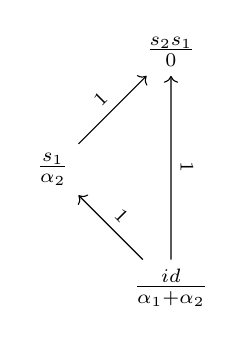
\begin{tikzpicture}[scale=1.5]
		\node (11) at (2,3) {$\frac{s_2 s_1}{0}$};
		\node (10) at (1,2) {$\frac{s_1}{\alpha_2}$};
		\node (00) at (2,1) {$\frac{id}{\alpha_1+\alpha_2}$};
		\draw[->] (00) -- (10) node [pos=0.50,  above, sloped] {$_{1}$};
		\draw[->] (00) -- (11) node [pos=0.50,  above, sloped] {$_{1}$};
		\draw[->] (10) -- (11) node [pos=0.50,  above, sloped] {$_{1}$};
	\end{tikzpicture}
\end{center}
\end{example}
\begin{example}\label{ex:A2} Consider $G=\mathrm{SL}_3(\mathbb{C})$ and $P=B$. In this case
$G/B= \mathrm{Fl}(3)$, the flag variety parametrizing complete flags $(F_1 \subset F_2 \subset \mathbb{C}^3)$. 
Set $v\coloneqq id$ and $w\coloneqq w_0 = s_1 s_2 s_1$ and consider two functions $\Lambda_i: W \to X^*(T)^+$ defined by:
\[ \Lambda_1(x) = \begin{cases} \varpi_1 & \textrm{if } x \neq s_2 s_1 \/; \\ \varpi_2 & \textrm{if } x = s_2 s_1 \/. \end{cases}
\quad \quad 
\Lambda_2(x) \equiv n_1 \varpi_1 + n_2 \varpi_2 \/, \quad (n_1, n_2 >0) \/.\]
One may easily check that both are admissible functions. The corresponding $\Lambda_i$-Bruhat graphs for the triple $(id,w_0,\Lambda_i)$ are below, from left to right.
\begin{center}
\begin{minipage}{4.75cm}
	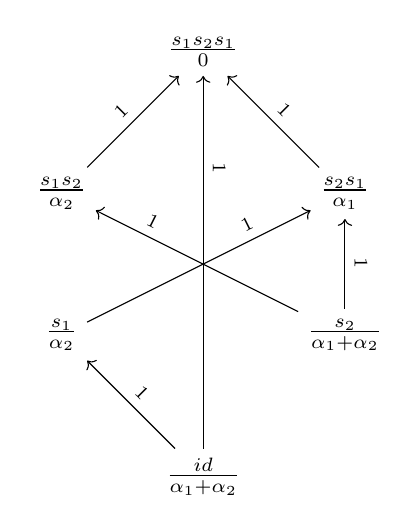
\begin{tikzpicture}[scale=0.9]
		\node (v0) at (3,6){$\frac{s_1 s_2 s_1}{0}$};
		\node (v1) at (1,4){$\frac{s_1 s_2}{\alpha_2}$};
		\node (v2) at (5,4){$\frac{s_2 s_1}{\alpha_1}$};
		\node (v3) at (1,2){$\frac{s_1}{\alpha_2}$};
		\node (v4) at (5,2){$\frac{s_2}{\alpha_1+\alpha_2}$};
		\node (v5) at (3,0){$\frac{id}{\alpha_1+\alpha_2}$};
		
		\draw[<-] (v0)--(v1) node [pos=0.50,  above, sloped] {$_{1}$};
		\draw[<-] (v0)--(v2) node [pos=0.50,  above, sloped] {$_{1}$};
		\draw[<-] (v0)--(v5) node [pos=0.25,  above, sloped] {$_{1}$};
		\draw[<-] (v1)--(v4) node [pos=0.25,  above, sloped] {$_{1}$};
		\draw[<-] (v2)--(v3) node [pos=0.25,  above, sloped] {$_{1}$};
		\draw[<-] (v2)--(v4) node [pos=0.50,  above, sloped] {$_{1}$};
		\draw[<-] (v3)--(v5) node [pos=0.50,  above, sloped] {$_{1}$};
	\end{tikzpicture}
\end{minipage}
\hspace{1cm}
\begin{minipage}{6.31cm}
	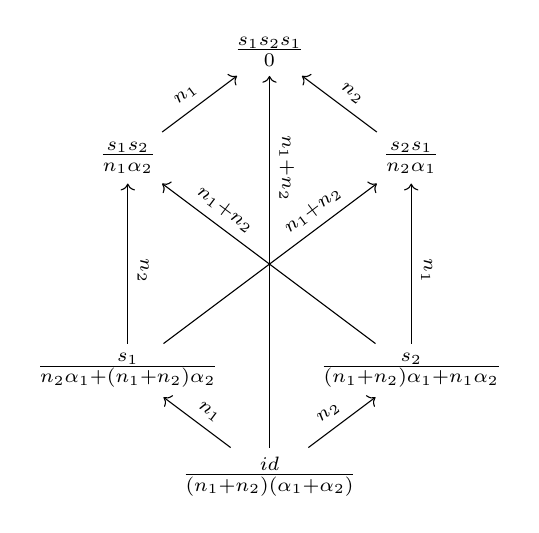
\begin{tikzpicture}[scale=0.9]
		\node (v0) at (3,6){$\frac{s_1 s_2 s_1}{0}$};
		\node (v1) at (1,4.5){$\frac{s_1 s_2}{n_1 \alpha_2}$};
		\node (v2) at (5,4.5){$\frac{s_2 s_1}{n_2 \alpha_1}$};
		\node (v3) at (1,1.5){$\frac{s_1}{n_2 \alpha_1 + (n_1 + n_2) \alpha_2}$};
		\node (v4) at (5,1.5){$\frac{s_2}{(n_1+n_2)\alpha_1+n_1 \alpha_2}$};
		\node (v5) at (3,0){$\frac{id}{(n_1+n_2)(\alpha_1 +\alpha_2)}$};
		
		\draw[<-] (v2) -- (v3) node [pos=0.25,  above, sloped] {$_{n_1+n_2}$};
		
		\draw[<-] (v1) -- (v4) node [pos=0.25, above, sloped] {$_{n_1+n_2}$};
		
		\draw[<-] (v0) -- (v5) node [pos=0.25, above, sloped] {$_{n_1+n_2}$} ;
		
		\draw[<-] (v0) -- (v1) node [pos=0.55,  above, sloped] {$_{n_1}$} ;
		
		\draw[<-] (v0) -- (v2)  node [pos=0.55,  above, sloped] {$_{n_2}$};
		
		\draw[<-] (v3) -- (v5)  node [pos=0.55,  above, sloped] {$_{n_1}$} ;
		
		\draw[<-] (v4) -- (v5)  node [pos=0.55,  above, sloped] {$_{n_2}$} ;
		
		\draw[<-] (v1) -- (v3)  node [pos=0.55, above, sloped] {$_{n_2}$};
		
		\draw[<-] (v2) -- (v4)  node [pos=0.55,  above, sloped] {$_{n_1}$} ;
	\end{tikzpicture}
\end{minipage}
\end{center}


\end{example}

\begin{example}\label{ex:B3} Consider the Lie type $B_3$, i.e.~$G = \mathrm{SO}(7,\mathbb{C})$.
The simple roots are $\Delta = \{ \alpha_1, \alpha_2, \alpha_3 \}$ with $\alpha_3$ short.~We choose 
$P$ to be the maximal parabolic determined by the set $\Delta_P = \{ \alpha_1, \alpha_3 \}$. 
Geometrically, $G/P$ is the submaximal isotropic Grassmannian
$\mathrm{IG}(2,7)$ parametrizing subspaces of dimension $2$ which 
are isotropic with respect to the non-degenerate symmetric 
form in $\mathbb{C}^7$. We pick the standard admissible function
$\Lambda(x) \equiv \varpi_2$ and $v=id,w=s_2 s_1 s_3 s_2$. All simple edges have Chevalley 
multiplicity $1$, and the double edges have multiplicity $2$.

Let us explain in more detail the calculations.
Each $u\in [id ,w]^P$ has $\ell(u)$ arrows directed to $u$. 
For example $w=s_2 s_1 s_3 s_2$ has four arrows
directed to $w$. 

\medskip

\noindent
\begin{minipage}{7.25cm}
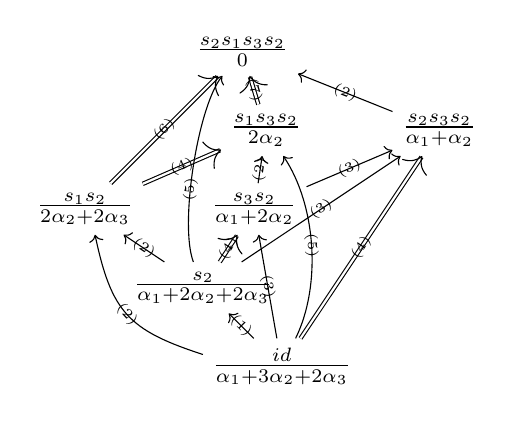
\begin{tikzpicture}[scale=0.5]
	\node (v0) at (10,8){$\frac{s_2 s_1 s_3 s_2}{0}$};
	\node (v1) at (10.6,6){$\frac{s_1 s_3 s_2}{2 \alpha_2}$};
	\node (v2) at (15,6){$\frac{s_2 s_3 s_2}{\alpha_1+\alpha_2}$};
	\node (v3) at (6,4){$\frac{s_1 s_2}{2\alpha_2+2 \alpha_3}$};
	\node (v4) at (10.3,4){$\frac{s_3 s_2}{\alpha_1+2\alpha_2}$};
	\node (v5) at (9,2){$\frac{s_2}{\alpha_1+2\alpha_2+2\alpha_3}$};
	\node (v6) at (11,0){$\frac{id}{\alpha_1+3\alpha_2+2\alpha_3}$};
	\draw[<-,double distance=0.8pt] (v0)-- node[pos=0.5,sloped]{\tiny\rm (7)}(v1);
	\draw[<-] (v0)--node[pos=0.5,sloped]{\tiny\rm (2)}(v2);
	\draw[<-,double distance=0.8pt] (v0)--node[pos=0.5,sloped]{\tiny\rm (6)}(v3);
	\draw[<-,double distance=0.8pt] (v1)--node[pos=0.5,sloped]{\tiny\rm (4)}(v3);
	\draw[<-] (v1)--node[pos=0.5,sloped]{\tiny\rm (2)}(v4);
	\draw[<-] (v2)--node[pos=0.5,sloped]{\tiny\rm (3)}(v4);
	\draw[<-] (v2)--node[pos=0.5,sloped]{\tiny\rm (3)}(v5);
	\draw[<-,double distance=0.8pt] (v2)--node[pos=0.5,sloped]{\tiny\rm (4)}(v6);
	\draw[<-] (v3)--node[pos=0.5,sloped]{\tiny\rm (2)}(v5);
	\draw[<-,double distance=0.8pt] (v4)--node[pos=0.5,sloped]{\tiny\rm (4)}(v5);
	\draw[<-] (v5)--node[pos=0.5,sloped]{\tiny\rm (1)}(v6);
	\draw[bend right,distance=2cm] (v3) to node[pos=0.5,sloped]{\tiny\rm (2)}(v6)[<-];
	\draw[<-] (v4)--node[pos=0.5,sloped]{\tiny\rm (3)}(v6);
	\draw[bend right,distance=1cm] (v0) to node[pos=0.6,sloped]{\tiny\rm (5)}(v5) [<-];
	\draw[bend left,distance=1.5cm] (v1) to node[pos=0.5,sloped]{\tiny\rm (5)}(v6)[<-];
\end{tikzpicture}
\end{minipage}
\hspace{-1.5cm}
{\begin{minipage}{7cm}
	
	\begin{center}
	We list below the reflections $s_\gamma$ \\
		s.t. $\langle\varpi_2,\gamma^\vee\rangle\neq 0$.
	\end{center}
	
	\scriptsize
	$
	\begingroup\setlength{\arraycolsep}{1pt}\begin{array}{c|c|c|c}
		no.&s_\gamma& \gamma&\gamma^\vee \\
		\hline
		(1)&s_2&\alpha_2&\alpha_2^\vee \\
		(2)&s_1s_2 s_1&\alpha_1+\alpha_2&a_1^\vee+a_2^\vee \\
		(3)&s_3 s_2 s_3&\alpha_2+2 \alpha_3&\alpha_2^\vee+a_3^\vee\\
		(4)&s_2 s_3 s_2&\alpha_2+ \alpha_3&2 \alpha_2^\vee+a_3^\vee\\
		(5)&s_3 s_2 s_1 s_2 s_3&\alpha_1+\alpha_2+ 2\alpha_3&\alpha_1^\vee+ \alpha_2^\vee+\alpha_3^\vee \\
		(6)&s_1 s_2 s_3 s_2 s_1&\alpha_1+\alpha_2+ \alpha_3&2 \alpha_1+2 \alpha_2^\vee+\alpha_3^\vee\\
		(7)&s_2 s_3 s_2 s_1 s_2 s_3 s_2&\alpha_1+2\alpha_2+ 2\alpha_3&\alpha_1^\vee+ 2\alpha_2^\vee+\alpha_3^\vee\\
	\end{array}\endgroup
	$
	\vspace{0.3cm}
	\normalsize
	$$
	\langle\varpi_2,\gamma^\vee\rangle=\begin{cases}
		1 & \text{ for } (1),(2),(3),(5)\\
		2 & \text{ for } (4),(6),(7)\\
	\end{cases}
	$$
	
	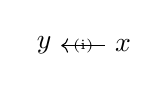
\begin{tikzpicture}[baseline=-1mm]
		\node (0) at (0,0) {$y$};
		\node (1) at (1,0) {$x$};
		\draw[<-] (0)--node[pos=0.5,sloped]{\tiny (i)}(1);
	\end{tikzpicture}
	indicates $x s_\gamma W_P=y W_P$, for (i)-th $s_\gamma$ in the above list.
	
\end{minipage}}

\end{example}





Next we record the following lemma.
\begin{lemma}\label{maxP} (a) Let $(v,w,\Lambda)$ be a  $\Lambda$-Bruhat graph and let $(x,y)$ be an edge such that
$yW_P = s_\beta x W_P = x s_\gamma W_P$. If $\Lambda(x)=\Lambda(y)=\lambda$ then
$x(\lambda) - y (\lambda) = m_\Lambda(x,y) \beta$.

(b) Let $\pi \in X(T)_P$ be a dominant integral weight and assume we are given a constant admissible function $\calW_\pi \equiv \pi$.
Then for any edge $x\overset{\beta}{\to} y$ as in (a) (with the notation from~\Cref{defin:order}): 
\begin{equation}\label{E:Wla} 
\mathcal{W}_\pi(x) = \mathcal{W}_\pi(y) + m_\pi(x,y) \beta \/.
\end{equation}
\end{lemma}
\begin{proof} 
By definition,
\begin{align*}
x(\lambda) - y (\lambda)=& x(\lambda)-xs_\gamma(\lambda)
=\langle \lambda,\gamma^\vee\rangle x(\gamma)
=m_\Lambda(x,y) \beta,
\end{align*}
where the last equality follows from \Cref{rem:gammabeta}. This proves part (a). Part (b) follows form (a) and 
the definition of $\calW_\pi$.\end{proof}

In the next section we will analyze $\Lambda$-Bruhat graphs for minuscule elements, and we will need the following 
result.
\begin{prop}\label{cor:multweight} Let $v < w$ be $\pi$-minuscule elements, and let $P$ be the parabolic 
subgroup defined by $W_P = Stab_W(\pi)$. Consider the 
$\Lambda$-Bruhat graph $(v,w,\Lambda)$ with 
the constant admissible function $\Lambda \equiv \pi$. Then the following hold:

(1) Let $x,y \in [v,w]^P$ be two elements and let $x \to y$ be an edge such that
$x W_P < y W_P = x s_\gamma W_P$. Then the Chevalley multiplicity 
satisfies:
\[ m_\pi(x,y) = \langle \pi, \gamma^\vee \rangle  =1 \/. \] 

(2) The $\Lambda\equiv \pi$-weight of the vertex $x$ (cf.~\Cref{def:ref_di}, parts (3) and (4)) is equal to: 
\[\mathcal{W}_\pi(x) = x(\pi) - w(\pi) = 
\sum_{i=0}^s \beta_i \quad \/, \]
where 
$x=x_0\overset{\beta_1}{\to} x_{1}\to \ldots \to x_{s-1}\overset{\beta_{s}}{\to} x_s =w$ 
is any chain in the $\Lambda$-Bruhat graph.

(3) The admissible function $\calW_\pi$ is injective.
\end{prop}
\begin{proof} By \Cref{lem:wminuscule}(2), since $w$ is $\pi$-minuscule, each element in 
$[v,w]^P$ is again 
$\pi$-minuscule. Let $\gamma'$ be the positive root such that $xW_P = y s_{\gamma'}W_P$ (cf.~\Cref{lemma:ubetav}).
From \Cref{rem:gammabeta}, the multiplicity
$m_\pi(x,y)$ is equal to $\langle \pi, (\gamma')^\vee \rangle$. Since $y s_{\gamma'} W_P < y W_P$ 
implies that $y s_{\gamma'} < y$, and since $y$ is $\pi$-minuscule,
$\langle \pi, (\gamma')^\vee \rangle = 1$ from \Cref{lem:gamma}. This proves part (1). 

From \Cref{maxP}(b) it follows that for any chain as in the hypothesis,
\[\calW_\pi(x) = x(\pi) - w(\pi) = \sum m_\pi(x_{i-1}, x_{i}) \beta_i \/. \]
Since by part (1) all multiplicities $m_\pi(x_{i-1}, x_{i})=1$, part (2) follows.
Finally, if $\calW_\pi(x) = \calW_\pi(y)$ then $x(\pi) = y(\pi)$, thus $x=y$ in $W^P$,
proving part (3).
\end{proof}


We now give a formula for the coefficients $d_{u,w}^w$ from \Cref{equ:CSMLR} in terms of summation 
over weighted paths in the $\Lambda$-Bruhat graph. 
\begin{prop}\label{prop:d_P}
For any $v\leq  w\in W^P$, fix an admissible function $\Lambda:[v,w]^P\to X^{*}(T)_P$, 
and let $\Gamma=(v,w,\Lambda)$ be the associated $\Lambda$-Bruhat graph. Then for $u\in [v,w]^P$,
\begin{equation}\label{eq:d}
d_{u,w}^w=\left(
\sum \frac{m_\Lambda(x_{r},x_{r-1})}{\mathcal{W}_\Lambda(x_{r})} \cdot \frac{m_\Lambda(x_{r-1},x_{r-2})}{\mathcal{W}_\Lambda(x_{r-1})}\cdot \ldots \cdot
\frac{m_\Lambda(x_1,x_0)}{\mathcal{W}_\Lambda(x_1)} \right)d_{w,w}^w .
\end{equation} where the sum is over integers $r \ge 0$, and over all directed paths 
$u= x_r \overset{}{\to} x_{r-1} \overset{}{\to} \ldots \overset{}{\to} x_0 = w$ in $\Gamma$. 
\end{prop}

\begin{proof}
There is nothing to do when $u=w$. If $u<w$, set $\lambda_u\coloneqq  \Lambda(u)$. Then from
\Cref{eq:recLR},
\[ \begin{split} d_{u,w}^w & = \frac{1}{w(\lambda_u) - u(\lambda_u)} \sum_{u < x} c_{\lambda_u, u}^x d_{x,w}^w
= \frac{1}{w(\lambda_u) - u(\lambda_u)} \sum_{x= us_\alpha >u ; \alpha >0} 
c_{\lambda_u, u}^x d_{x,w}^w
\\ & = \frac{1}{w(\lambda_u) - u(\lambda_u)} \sum_{x= us_\alpha >u ; \alpha >0} \langle -\lambda_u , \alpha^\vee \rangle  d_{x,w}^w = 
\frac{1}{\mathcal{W}_\Lambda(u)} \sum_{u \overset{}{\to} x } m_\Lambda(u,x) d_{x,w}^w \\ &
= \sum_{u \overset{}{\to} x } \frac{m_\Lambda(u,x)}{\mathcal{W}_\Lambda(u)} d_{x,w}^w \/. \end{split}
\] Here the second equality follows from \Cref{thm:chevalley} and the definition of $c_{\lambda, u}^x$ in \Cref{equ:ccoeff}, and the rest are from the definitions. Then the statement follows
by induction descending from $w$, on those elements $x$ such that $u<x\le w$.
\end{proof}
From \Cref{lem:CSMLR} we deduce another interpretation of the sum in the previous proposition:
\begin{corol}\label{thm:LocCSM2} Let $v \le w$ be two elements in $W^P$. 
With the hypotheses from \Cref{prop:d_P}, the following hold:
\begin{equation}\label{hook-formula}
\frac{\ssm(Y(v))|_w}{\ssm(Y(w))|_w} =
\sum
\frac{m_\Lambda(x_r,x_{r-1})}{\mathcal{W}_\Lambda(x_r)}\cdot \frac{m_\Lambda(x_{r-1},x_{r-2})}{\mathcal{W}_\Lambda(x_{r-1})}\cdot \ldots \cdot \frac{m_\Lambda(x_{1},x_{0})}{\mathcal{W}_\Lambda(x_{1})},
\end{equation} where the sum is over integers $r \ge 0$, and over all directed paths 
$v\leq x_r \overset{}{\to} x_{r-1} \overset{}{\to} \ldots \overset{}{\to} x_0 = w$ in $\Gamma$.
\end{corol}
\begin{proof} By \Cref{lem:CSMLR} and the additivity of CSM classes, 
the left hand side of \eqref{hook-formula} is equal to 
\[\displaystyle \frac{\ssm(Y(v))|_w}{\ssm(Y(w))|_w}=\frac{\sum_{v\leq u}\ssm(Y(u)^\circ)|_w}{\ssm(Y(w)^\circ)|_w} =\sum_{v\leq u\leq w} \frac{d_{u,w}^{w}}{d_{w,w}^{w}}
\/.
\] 
Here we also used that $\ssm(Y(u)^\circ)|_w=0$ if $w \ngeq u$.
Then the claim follows from \Cref{prop:d_P}.\end{proof}

\begin{remark} By \Cref{prop:loc} and \Cref{prop:eqmult}, the left hand side of \Cref{hook-formula} 
is an equivariant multiplicity, which may be calculated explicitly. Fix a reduced expression $w=s_{i_1} s_{i_2} \cdots s_{i_\ell}$
and set $\beta_j=s_{i_1} s_{i_2} \cdots s_{i_{j-1}}(\alpha_{i_j})$
$(j=1,2,\ldots,\ell)$. Then:
\begin{equation}\label{equ:explicit} \frac{\ssm(Y(v))|_w}{\ssm(Y(w))|_w} = 
e_{w,G/P}(\csm(R_w^v)) =\frac{\sum \beta_{j_1}\beta_{j_2}\cdot \ldots \cdot \beta_{j_k}}{\beta_1\cdot \ldots \cdot \beta_\ell} \/;
\end{equation}
here 
the summation is over $ 1\leq j_1<j_2<\cdots <j_k\leq \ell$ such that 
$vW_P\leq s_{i_{j_1}}s_{i_{j_2}}\cdots s_{i_{j_k}}W_P$.

As we observed in \Cref{thm:smoothP}, if $Y(v)$ is smooth at $wP$, then 
both the numerator and the denominator of this expression may be written as products.
This is the key observation which leads to a generalization of Nakada's hook formula in the next section.\end{remark}


\section{A generalized colored hook formula}\label{sec:genhook}
In this section we prove the main result of this paper - 
the generalization of Nakada's colored hook formula, together with several corollaries 
of it.
\subsection{The colored hook formula and consequences}\label{sec:col-and-conseq}
Recall that for $v < w \in W$, $S(w/v)\coloneqq \{\beta\in R^+\mid v\le s_\beta w<w\}$.
\begin{theorem}\label{thm:genNak} Let $v\leq  w\in W^P$, and fix an admissible 
	function $\Lambda:[v,w]^P\to X^{*}(T)_P$ with the associated 
	$\Lambda$-Bruhat graph $\Gamma=(v,w,\Lambda)$. Then: 
	\begin{center}
		$Y(v)\subset G/P$ is smooth at $wP\in G/P$  if and only if
		\[
		\sum\frac{m_\Lambda(x_r,x_{r-1})}{\mathcal{W}_\Lambda(x_r)}\cdot \frac{m_\Lambda(x_{r-1},x_{r-2})}{\mathcal{W}_\Lambda(x_{r-1})}\cdot \ldots \cdot \frac{m_\Lambda(x_{1},x_{0})}{\mathcal{W}_\Lambda(x_{1})}
		\;=\;
		\prod_{\beta \in S(w/v)} \left(1+\frac{1}{\beta}\right),\]
	\end{center}
	where the sum is over integers $r \ge 0$, and over all directed paths 
	$v\leq x_r \overset{}{\to} x_{r-1} \overset{}{\to} \ldots \overset{}{\to} x_0 = w$ in $\Gamma$.
\end{theorem}

\begin{proof} We proved in \Cref{prop:eqmult} that 
	\[ \frac{\ssm(Y(v))|_w}{\ssm(Y(w))|_w}=e_{w,G/P} (\csm(R_w^{v})) \/. \]
	Then by 
	\Cref{thm:smoothP}, $Y(v)\subset G/P$ is smooth at $wP\in G/P$ if and only if 
	\[ \frac{\ssm(Y(v))|_w}{\ssm(Y(w))|_w} = \prod_{\beta\in S(w/v)}(1+\frac{1}{\beta}) \/. \]
	Now observe that by \Cref{thm:LocCSM2} the left hand side of this expression is the sum in the statement.\end{proof}
An important particular case of \Cref{thm:genNak} is to consider a constant admissible function.
For example, let $\pi\in X^*(T)$ be any dominant integral weight, and as usual define 
$P$ by $\Stab_W(\pi)=W_P$. Set
$\Lambda(x) \equiv \pi$ for $x \in [v,w]^P$, and recall that $\calW_\pi$ denotes the associated
weight function. Let $m_i = \langle \pi, \gamma_i^\vee \rangle$ be the multiplicity of the 
edge $x_i \to x_{i-1}$ and let $\beta_i$ be the positive root
$\beta_i$ such that $x_{i-1}W_P = s_{\beta_i}x_i W_P$.
With this notation, and by \Cref{thm:genNak}, we deduce the following.
\begin{corol}\label{col:NakP}
	Under the above assumptions,
	we have the following equivalence:
	\begin{center}
		$Y(v)\subset G/P$ is smooth at $wP\in G/P$  if and only if
		\[
		\sum \frac{m_r}{m_1\beta_1+m_2\beta_2+\cdots +m_r\beta_r} \cdot \ldots \cdot 
		\frac{m_1}{m_1\beta_1}
		=\prod_{\beta \in S(w/v)}\left(1+\frac{1}{\beta}\right),
		\]
	\end{center}
	where the sum is over all integers $r \ge 0$, and over all directed paths 
	$v\leq x_r \overset{\beta_r}{\to} x_{r-1} \overset{\beta_{r-1}}{\to} \ldots \overset{\beta_1}{\to} x_0 = w$ in $\Gamma= (v,w,\pi)$. 
\end{corol}
\begin{proof} Immediate from \Cref{thm:genNak}, since $\mathcal{W}_\pi(x_k)=\sum_{i=1}^k m_i \beta_i$,
	by \Cref{E:Wla}. 
\end{proof}


\begin{corol}\label{col:Nak} 
	Let $v \le w \in W$ be two $\pi$-minuscule elements for a dominant integral weight $\pi$,
	and $P\subset G$ be the parabolic subgroup satisfying 
	$\Stab_W(\pi)=W_P$. Then: 
	\begin{center}
		$Y(v)\subset G/P$ is smooth at $wP\in G/P$  if and only if
		\begin{equation}\label{E:minusculeNak}
			\sum \frac{1}{\beta_1+\beta_2+\cdots +\beta_r} \cdot \ldots \cdot 
			\frac{1}{\beta_1}
			=\prod_{\beta \in S(w/v)}\left(1+\frac{1}{\beta}\right),
		\end{equation}
	\end{center}
	where the sum is as in \Cref{col:NakP}.
\end{corol}
\begin{proof} First observe that by \Cref{lem:wminuscule}(2), 
	since $w$ is $\pi$-minuscule, each representative $x \in W^P$ in a chain to $w$ 
	is also $\pi$-minuscule. Then from \Cref{col:NakP}, we only need to show that 
	any edge $x \to y$ has multiplicity $m_\pi(x,y)=1$. This follows from \Cref{cor:multweight}.
\end{proof}
If $v=id$, \Cref{col:Nak} recovers Nakada's colored hook formula stated in \Cref{thm:anotherform}. 

\Cref{col:Nak} implies 
a skew version of the classical Peterson formula~\cite{carrell:vector,proctor:minuscule};
see also~\cite{kleschchev.ram} for related recent work in this direction.

Recall that $\Red(w)$ 
denotes the set of all reduced expressions of $w$ and $\h(\beta)$ is the height of the positive root $\beta$ (see \S\ref{sec:prelims}).
\begin{corol}[A skew Peterson formula]\label{cor:skewPP} Let $\pi$ be a 
	dominant integral weight, and let $P$ be the parabolic subgroup defined by
	$\Stab_W(\pi)=W_P$. Let $v \le w\in W$ be $\pi$-minuscule elements 
	such that
	$Y(vW_P)$ is smooth at $wP$. Then
	\begin{equation}\label{equ:petersonproctor}
		\#\Red(wv^{-1})=\frac{(\ell(w)-\ell(v))!}{\prod_{\beta\in S(w/v)}\h(\beta)} ~\/.
	\end{equation}
\end{corol}
\begin{proof} Consider the term of lowest degree $-\# S(w/v)$ in the expression in \Cref{col:Nak}. This corresponds to taking the summation over {\em maximal paths} in \Cref{col:Nak}, and yields
	\begin{equation}\label{eq:max_path}
		\sum \frac{1}{\beta_1+\beta_2+\cdots +\beta_r} \cdot \ldots \cdot 
		\frac{1}{\beta_1}
		=\prod_{\beta \in S(w/v)} \frac{1}{\beta} \/.
	\end{equation}
	The paths considered are the same as the paths from \Cref{cor:skewred}, in particular each $\beta_i$ 
	is a simple root. Now specialize each simple root $\alpha_i \mapsto 1$. The right hand side gives $\frac{1}{\prod_{\beta\in S(w/v)}\h(\beta)}$. On the left hand side, each summand specializes to $\frac{1}{ (\ell(w)-\ell(v)) !}$, and the number of summands is equal to the number of reduced expressions of $wv^{-1}$, again by 
	\Cref{cor:skewred}.\end{proof}

\begin{remark}\label{rem:reducetoid} One can show that in the hypotheses
	from \Cref{col:Nak}, and if $W$ is a simply laced Weyl group, then 
	then $Y(v)$ is smooth at $w$ if and only if $wv^{-1}$ is $\pi'$-minuscule, 
	where $\pi'$ is dominant integral. Furthermore, in this case the identities~\eqref{E:minusculeNak} and \eqref{equ:petersonproctor}
	for $[v,w]^\pi$ coincide with those corresponding to the interval $[id,wv^{-1}]^{\pi'}$.
	The proof requires developing techniques different from those employed in 
		this paper and will appear in a separate note.
	
	If $W$ is not simply laced then it is possible that $Y(v)$ is smooth at $w$, but $wv^{-1}$ is not dominant minuscule. An 
	example is in type $F_4$ for $v=s_1$, $w=s_1 s_3 s_2s_4s_3s_2s_1$, with $\alpha_1, \alpha_2$ short roots. However, in this case one can 
	show that if $Y(v)$ is smooth at $w$,
	the `skew' Nakada's identity is obtained from the `straight' formula applied to suitable elements 
	in type $E_6$. The transformation between the two cases is given by the folding of the root system
	$E_6$ into $F_4$. This suggests that folding may lead to a more general statement relating skew and straight Nakada formulae. 
\end{remark}



\begin{remark}\label{rem:general_miuscule} Let $w$ be dominant minuscule and 
		$v\in [id,w]^P$. If we remove the condition that $Y(vW_P)$ is smooth at $wP$, by equations \eqref{hook-formula}, \eqref{equ:explicit}, and the proof of \Cref{cor:skewPP}, 
	we obtain
	\begin{equation}\label{skew:cohomology}
		\# \Red(wv^{-1})=(\ell(w)-\ell(v))!\frac{\sum \h(\beta_{j_1})\h(\beta_{j_2})\cdots \h(\beta_{j_{\ell(v)}})}{\h(\beta_1)\cdots \h(\beta_\ell)}
	\end{equation}
	where the summation is over $ 1\leq j_1<j_2<\cdots <\ell(v)\leq \ell$ such that 
	$v= s_{i_{j_1}}s_{i_{j_2}}\cdots s_{i_{j_{\ell(v)}}}$ is a reduced decomposition. 
	
	Observe also that the right hand side is the specialization of
	$(\ell(w)-\ell(v))!\frac{[Y(v)]|_w}{[Y(w)]|_w}$ 
	by taking a root to its height.
	To relate to the right hand side in \Cref{thm:genNak}, observe that 
		the fraction $\frac{[Y(v)]|_w}{[Y(w)]|_w}$
		may also be obtained by taking the lowest degree terms in the numerator and denominator of
		the fraction $\frac{\ssm(Y(v))|_w}{\ssm(Y(w))|_w}$.
		This fact follows from \Cref{prop:loc} above, or, more directly, 
		because the Segre class satisfies: 
		\[ \ssm(Y(v)) = [Y(v)] + \textrm{ higher order terms in $H^*_T(G/P)$} \/.\]
\end{remark}

\begin{thebibliography}{MMMMMM}
\bibitem[1]{AMSS:shadows} Aluffi, Paolo; Mihalcea, Leonardo C.; Schürmann, Jörg; Su, Changjian Shadows of characteristic cycles, Verma modules, and positivity of Chern–Schwartz–MacPherson classes of Schubert cells, Duke Math. J., Volume 172 (2023) no. 17, pp. 3257-3320 \href{https://alco.centre-mersenne.org/articles/10.5802/alco.428/#AMSS:shadows}{Publisher reference}.
\bibitem[2]{AMSS:motivic} Aluffi, Paolo; Mihalcea, Leonardo C.; Schürmann, Jörg; Su, Changjian Motivic Chern classes of Schubert cells, Hecke algebras, and applications to Casselman’s problem, Ann. Sci. Éc. Norm. Supér. (4), Volume 57 (2024) no. 1, pp. 87-141 \href{https://alco.centre-mersenne.org/articles/10.5802/alco.428/#AMSS:motivic}{Publisher reference}.
\bibitem[3]{billey.coskun:singularities} Billey, Sara; Coskun, Izzet Singularities of generalized Richardson varieties, Comm. Algebra, Volume 40 (2012) no. 4, pp. 1466-1495 \href{https://alco.centre-mersenne.org/articles/10.5802/alco.428/#billey.coskun:singularities}{Publisher reference}.
\bibitem[4]{bourbaki:Lie4-6} Bourbaki, Nicolas Lie groups and Lie algebras. Chapters 4–6, Elements of Mathematics (Berlin), Springer-Verlag, Berlin, 2002, xii+300 pages (translated from the 1968 French original by Andrew Pressley) \href{https://alco.centre-mersenne.org/articles/10.5802/alco.428/#bourbaki:Lie4-6}{Publisher reference}.
\bibitem[5]{BS81} Brasselet, Jean-Paul; Schwartz, Marie-Hélène Sur les classes de Chern d’un ensemble analytique complexe, The Euler-Poincaré characteristic (French) (Astérisque), Volume 82-83, Soc. Math. France, Paris, 1981, pp. 93-147 \href{https://alco.centre-mersenne.org/articles/10.5802/alco.428/#BS81}{Publisher reference}.
\bibitem[6]{BFP99} Brenti, Francesco; Fomin, Sergey; Postnikov, Alexander Mixed Bruhat operators and Yang–Baxter equations for Weyl groups, Internat. Math. Res. Notices (1999) no. 8, pp. 419-441 \href{https://alco.centre-mersenne.org/articles/10.5802/alco.428/#BFP99}{Publisher reference}.
\bibitem[7]{brion:eq-chow} Brion, Michel Equivariant Chow groups for torus actions, Transform. Groups, Volume 2 (1997) no. 3, pp. 225-267 \href{https://alco.centre-mersenne.org/articles/10.5802/alco.428/#brion:eq-chow}{Publisher reference}.
\bibitem[8]{BCMP:QKChev} Buch, Anders S.; Chaput, Pierre-Emmanuel; Mihalcea, Leonardo C.; Perrin, Nicolas A Chevalley formula for the equivariant quantum K-theory of cominuscule varieties, Algebr. Geom., Volume 5 (2018) no. 5, pp. 568-595 \href{https://alco.centre-mersenne.org/articles/10.5802/alco.428/#BCMP:QKChev}{Publisher reference}.
\bibitem[9]{buch.m:nbhds} Buch, Anders S.; Mihalcea, Leonardo C. Curve neighborhoods of Schubert varieties, J. Differential Geom., Volume 99 (2015) no. 2, pp. 255-283 \href{https://alco.centre-mersenne.org/articles/10.5802/alco.428/#buch.m:nbhds}{Publisher reference}.
\bibitem[10]{carrell:vector} Carrell, James B. Vector fields, flag varieties and Schubert calculus, Proceedings of the Hyderabad Conference on Algebraic Groups (Hyderabad, 1989), Manoj Prakashan, Madras (1991), pp. 23-57 \href{https://alco.centre-mersenne.org/articles/10.5802/alco.428/#carrell:vector}{Publisher reference}.
\bibitem[11]{carrell:bruhat} Carrell, James B. The Bruhat graph of a Coxeter group, a conjecture of Deodhar, and rational smoothness of Schubert varieties, Algebraic groups and their generalizations: classical methods (University Park, PA, 1991) (Proc. Sympos. Pure Math.), Volume 56, Part 1, Amer. Math. Soc., Providence, RI, 1994, pp. 53-61 \href{https://alco.centre-mersenne.org/articles/10.5802/alco.428/#carrell:bruhat}{Publisher reference}.
\bibitem[12]{Cas19} Casbi, Elie Equivariant multiplicities of simply-laced type flag minors, Represent. Theory, Volume 25 (2021), pp. 1049-1092 \href{https://alco.centre-mersenne.org/articles/10.5802/alco.428/#Cas19}{Publisher reference}.
\bibitem[13]{casbi2019newton} Casbi, Elie Newton-Okounkov bodies for categories of modules over quiver Hecke algebras, Ann. Inst. Fourier (Grenoble), Volume 72 (2022) no. 5, pp. 1773-1818 \href{https://alco.centre-mersenne.org/articles/10.5802/alco.428/#casbi2019newton}{Publisher reference}.
\bibitem[14]{edidin.graham:eqchow} Edidin, Dan; Graham, William Equivariant intersection theory, Invent. Math., Volume 131 (1998) no. 3, pp. 595-634 \href{https://alco.centre-mersenne.org/articles/10.5802/alco.428/#edidin.graham:eqchow}{Publisher reference}.
\bibitem[15]{edidin-graham:localization} Edidin, Dan; Graham, William Localization in equivariant intersection theory and the Bott residue formula, Amer. J. Math., Volume 120 (1998) no. 3, pp. 619-636 \href{https://alco.centre-mersenne.org/articles/10.5802/alco.428/#edidin-graham:localization}{Publisher reference}.
\bibitem[16]{fulton.woodward} Fulton, W.; Woodward, C. On the quantum product of Schubert classes, J. Algebraic Geom., Volume 13 (2004) no. 4, pp. 641-661 \href{https://alco.centre-mersenne.org/articles/10.5802/alco.428/#fulton.woodward}{Publisher reference}.
\bibitem[17]{fulton:IT} Fulton, William Intersection theory, Ergebnisse der Mathematik und ihrer Grenzgebiete. 3. Folge. A Series of Modern Surveys in Mathematics, 2, Springer-Verlag, Berlin, 1998, xiv+470 pages \href{https://alco.centre-mersenne.org/articles/10.5802/alco.428/#fulton:IT}{Publisher reference}.
\bibitem[18]{graham.kreiman:excited} Graham, William; Kreiman, Victor Excited Young diagrams, equivariant K-theory, and Schubert varieties, Trans. Amer. Math. Soc., Volume 367 (2015) no. 9, pp. 6597-6645 \href{https://alco.centre-mersenne.org/articles/10.5802/alco.428/#graham.kreiman:excited}{Publisher reference}.
\bibitem[19]{graham.kreiman:cominuscule_pt} Graham, William; Kreiman, Victor Cominuscule points and Schubert varieties, Ann. Inst. Fourier (Grenoble), Volume 71 (2021) no. 6, pp. 2519-2548 \href{https://alco.centre-mersenne.org/articles/10.5802/alco.428/#graham.kreiman:cominuscule_pt}{Publisher reference}.
\bibitem[20]{ikeda2009excited} Ikeda, Takeshi; Naruse, Hiroshi Excited Young diagrams and equivariant Schubert calculus, Trans. Amer. Math. Soc., Volume 361 (2009) no. 10, pp. 5193-5221 \href{https://alco.centre-mersenne.org/articles/10.5802/alco.428/#ikeda2009excited}{Publisher reference}.
\bibitem[21]{Kaw15} Kawanaka, Noriaki Games and algorithms with hook structure, Sugaku Expositions, Volume 28 (2015) no. 1, pp. 73-93 (translated from the Japanese) \href{https://alco.centre-mersenne.org/articles/10.5802/alco.428/#Kaw15}{Publisher reference}.
\bibitem[22]{kleschchev.ram} Kleshchev, Alexander; Ram, Arun Homogeneous representations of Khovanov-Lauda algebras, J. Eur. Math. Soc. (JEMS), Volume 12 (2010) no. 5, pp. 1293-1306 \href{https://alco.centre-mersenne.org/articles/10.5802/alco.428/#kleschchev.ram}{Publisher reference}.
\bibitem[23]{knutson.tao:puzzles} Knutson, Allen; Tao, Terence Puzzles and (equivariant) cohomology of Grassmannians, Duke Math. J., Volume 119 (2003) no. 2, pp. 221-260 \href{https://alco.centre-mersenne.org/articles/10.5802/alco.428/#knutson.tao:puzzles}{Publisher reference}.
\bibitem[24]{kumar1996nil} Kumar, Shrawan The nil Hecke ring and singularity of Schubert varieties, Invent. Math., Volume 123 (1996) no. 3, pp. 471-506 \href{https://alco.centre-mersenne.org/articles/10.5802/alco.428/#kumar1996nil}{Publisher reference}.
\bibitem[25]{kumar:book} Kumar, Shrawan Kac–Moody groups, their flag varieties and representation theory, Progress in Mathematics, 204, Birkhäuser Boston, Inc., Boston, MA, 2002, xvi+606 pages \href{https://alco.centre-mersenne.org/articles/10.5802/alco.428/#kumar:book}{Publisher reference}.
\bibitem[26]{LNSSS} Lenart, Cristian; Naito, Satoshi; Sagaki, Daisuke; Schilling, Anne; Shimozono, Mark A uniform model for Kirillov–Reshetikhin crystals I: Lifting the parabolic quantum Bruhat graph, Int. Math. Res. Not. IMRN, Volume 2015 (2015) no. 7, pp. 1848-1901 \href{https://alco.centre-mersenne.org/articles/10.5802/alco.428/#LNSSS}{Publisher reference}.
\bibitem[27]{macpherson:chern} MacPherson, Robert D. Chern classes for singular algebraic varieties, Ann. of Math. (2), Volume 100 (1974), pp. 423-432 \href{https://alco.centre-mersenne.org/articles/10.5802/alco.428/#macpherson:chern}{Publisher reference}.
\bibitem[28]{mihalcea:eqqgr} Mihalcea, Leonardo Equivariant quantum Schubert calculus, Adv. Math., Volume 203 (2006) no. 1, pp. 1-33 \href{https://alco.centre-mersenne.org/articles/10.5802/alco.428/#mihalcea:eqqgr}{Publisher reference}.
\bibitem[29]{mihalcea2020left} Mihalcea, Leonardo C.; Naruse, Hiroshi; Su, Changjian Left Demazure-Lusztig operators on equivariant (quantum) cohomology and K-theory, Int. Math. Res. Not. IMRN (2022) no. 16, pp. 12096-12147 \href{https://alco.centre-mersenne.org/articles/10.5802/alco.428/#mihalcea2020left}{Publisher reference}.
\bibitem[30]{MNS24Coxeterhook} Mihalcea, Leonardo C.; Naruse, Hiroshi; Su, Changjian Hook formula for Coxeter groups via the twisted group ring, Proc. Japan Acad. Ser. A Math. Sci., Volume 100 (2024) no. 6, pp. 31-36 \href{https://alco.centre-mersenne.org/articles/10.5802/alco.428/#MNS24Coxeterhook}{Publisher reference}.
\bibitem[31]{mihalcea:eqqhom} Mihalcea, Leonardo Constantin On equivariant quantum cohomology of homogeneous spaces: Chevalley formulae and algorithms, Duke Math. J., Volume 140 (2007) no. 2, pp. 321-350 \href{https://alco.centre-mersenne.org/articles/10.5802/alco.428/#mihalcea:eqqhom}{Publisher reference}.
\bibitem[32]{molev.sagan:Littlewood-Richardson} Molev, Alexander I.; Sagan, Bruce E. A Littlewood-Richardson rule for factorial Schur functions, Trans. Amer. Math. Soc., Volume 351 (1999) no. 11, pp. 4429-4443 \href{https://alco.centre-mersenne.org/articles/10.5802/alco.428/#molev.sagan:Littlewood-Richardson}{Publisher reference}.
\bibitem[33]{morales.pak.panovaLhook} Morales, Alejandro H.; Pak, Igor; Panova, Greta Hook formulas for skew shapes I. q-analogues and bijections, J. Combin. Theory Ser. A, Volume 154 (2018), pp. 350-405 \href{https://alco.centre-mersenne.org/articles/10.5802/alco.428/#morales.pak.panovaLhook}{Publisher reference}.
\bibitem[34]{nakada:colored} Nakada, Kento Colored hook formula for a generalized Young diagram, Osaka J. Math., Volume 45 (2008) no. 4, pp. 1085-1120 \href{https://alco.centre-mersenne.org/articles/10.5802/alco.428/#nakada:colored}{Publisher reference}.
\bibitem[35]{nakada:proc} Nakada, Kento A hook formula for the standard tableaux of a generalized shape, Combinatorial representation theory and related topics (RIMS Kôkyûroku Bessatsu, B8), Res. Inst. Math. Sci. (RIMS), Kyoto, 2008, pp. 55-62 \href{https://alco.centre-mersenne.org/articles/10.5802/alco.428/#nakada:proc}{Publisher reference}.
\bibitem[36]{naruse2014schubert} Naruse, Hiroshi Schubert calculus and hook formula, slides at the 73rd Sém. Lothar. Combin., Strobl, Austria, 2014 \url{https://www.emis.de/...} \href{https://alco.centre-mersenne.org/articles/10.5802/alco.428/#naruse2014schubert}{Publisher reference}.
\bibitem[37]{naruse2019skew} Naruse, Hiroshi; Okada, Soichi Skew hook formula for d-complete posets via equivariant K-theory, Algebr. Comb., Volume 2 (2019) no. 4, pp. 541-571 \href{https://alco.centre-mersenne.org/articles/10.5802/alco.428/#naruse2019skew}{Publisher reference}.
\bibitem[38]{ohmoto:eqcsm} Ohmoto, Toru Equivariant Chern classes of singular algebraic varieties with group actions, Math. Proc. Cambridge Philos. Soc., Volume 140 (2006) no. 1, pp. 115-134 \href{https://alco.centre-mersenne.org/articles/10.5802/alco.428/#ohmoto:eqcsm}{Publisher reference}.
\bibitem[39]{panova.petrov:hook} Panova, Greta; Petrov, Leonid Hook-length Formulas for Skew Shapes via Contour Integrals and Vertex Models, 2024 \href{https://alco.centre-mersenne.org/articles/10.5802/alco.428/#panova.petrov:hook}{Publisher reference}.
\bibitem[40]{proctor:bruhat} Proctor, Robert A. Bruhat lattices, plane partition generating functions, and minuscule representations, European J. Combin., Volume 5 (1984) no. 4, pp. 331-350 \href{https://alco.centre-mersenne.org/articles/10.5802/alco.428/#proctor:bruhat}{Publisher reference}.
\bibitem[41]{proctor:dynkin} Proctor, Robert A. Dynkin diagram classification of λ-minuscule Bruhat lattices and of d-complete posets, J. Algebraic Combin., Volume 9 (1999) no. 1, pp. 61-94 \href{https://alco.centre-mersenne.org/articles/10.5802/alco.428/#proctor:dynkin}{Publisher reference}.
\bibitem[42]{proctor:minuscule} Proctor, Robert A. Minuscule elements of Weyl groups, the numbers game, and d-complete posets, J. Algebra, Volume 213 (1999) no. 1, pp. 272-303 \href{https://alco.centre-mersenne.org/articles/10.5802/alco.428/#proctor:minuscule}{Publisher reference}.
\bibitem[43]{schurmann:transversality} Schürmann, Jörg Chern classes and transversality for singular spaces, Singularities in geometry, topology, foliations and dynamics (Trends Math.), Birkhäuser/Springer, Cham, 2017, pp. 207-231 \href{https://alco.centre-mersenne.org/articles/10.5802/alco.428/#schurmann:transversality}{Publisher reference}.
\bibitem[44]{schurmann.simpson.wang} Schürmann, Jörg; Simpson, Connor; Wang, Botong A new generic vanishing theorem on homogeneous varieties and the positivity conjecture for triple intersections of Schubert cells, Compos. Math., Volume 161 (2025) no. 1, pp. 1-12 \href{https://alco.centre-mersenne.org/articles/10.5802/alco.428/#schurmann.simpson.wang}{Publisher reference}.
\bibitem[45]{schwartz:1} Schwartz, Marie-Hélène Classes caractéristiques définies par une stratification d’une variété analytique complexe. I, C. R. Acad. Sci. Paris, Volume 260 (1965), pp. 3262-3264 \href{https://alco.centre-mersenne.org/articles/10.5802/alco.428/#schwartz:1}{Publisher reference}.
\bibitem[46]{schwartz:2} Schwartz, Marie-Hélène Classes caractéristiques définies par une stratification d’une variété analytique complexe. II, C. R. Acad. Sci. Paris, Volume 260 (1965), pp. 3535-3537 \href{https://alco.centre-mersenne.org/articles/10.5802/alco.428/#schwartz:2}{Publisher reference}.
\bibitem[47]{stanley:reduced} Stanley, Richard P. On the number of reduced decompositions of elements of Coxeter groups, European J. Combin., Volume 5 (1984) no. 4, pp. 359-372 \href{https://alco.centre-mersenne.org/articles/10.5802/alco.428/#stanley:reduced}{Publisher reference}.
\bibitem[48]{stembridge:fullycomm} Stembridge, John R. On the fully commutative elements of Coxeter groups, J. Algebraic Combin., Volume 5 (1996) no. 4, pp. 353-385 \href{https://alco.centre-mersenne.org/articles/10.5802/alco.428/#stembridge:fullycomm}{Publisher reference}.
\bibitem[49]{stembridge2001minuscule} Stembridge, John R. Minuscule elements of Weyl groups, J. Algebra, Volume 235 (2001) no. 2, pp. 722-743 \href{https://alco.centre-mersenne.org/articles/10.5802/alco.428/#stembridge2001minuscule}{Publisher reference}.
\bibitem[50]{su:quantum} Su, Changjian Equivariant quantum cohomology of cotangent bundle of G/P, Adv. Math., Volume 289 (2016), pp. 362-383 \href{https://alco.centre-mersenne.org/articles/10.5802/alco.428/#su:quantum}{Publisher reference}.
\bibitem[51]{su:structure} Su, Changjian Structure constants for Chern classes of Schubert cells, Math. Z., Volume 298 (2021) no. 1-2, pp. 193-213 \href{https://alco.centre-mersenne.org/articles/10.5802/alco.428/#su:structure}{Publisher reference}.
\end{thebibliography}
\end{document}
